% Options for packages loaded elsewhere
\PassOptionsToPackage{unicode}{hyperref}
\PassOptionsToPackage{hyphens}{url}
\PassOptionsToPackage{dvipsnames,svgnames,x11names}{xcolor}
%
\documentclass[
]{interact}

\usepackage{amsmath,amssymb}
\usepackage{iftex}
\ifPDFTeX
  \usepackage[T1]{fontenc}
  \usepackage[utf8]{inputenc}
  \usepackage{textcomp} % provide euro and other symbols
\else % if luatex or xetex
  \usepackage{unicode-math}
  \defaultfontfeatures{Scale=MatchLowercase}
  \defaultfontfeatures[\rmfamily]{Ligatures=TeX,Scale=1}
\fi
\usepackage{lmodern}
\ifPDFTeX\else  
    % xetex/luatex font selection
\fi
% Use upquote if available, for straight quotes in verbatim environments
\IfFileExists{upquote.sty}{\usepackage{upquote}}{}
\IfFileExists{microtype.sty}{% use microtype if available
  \usepackage[]{microtype}
  \UseMicrotypeSet[protrusion]{basicmath} % disable protrusion for tt fonts
}{}
\makeatletter
\@ifundefined{KOMAClassName}{% if non-KOMA class
  \IfFileExists{parskip.sty}{%
    \usepackage{parskip}
  }{% else
    \setlength{\parindent}{0pt}
    \setlength{\parskip}{6pt plus 2pt minus 1pt}}
}{% if KOMA class
  \KOMAoptions{parskip=half}}
\makeatother
\usepackage{xcolor}
\setlength{\emergencystretch}{3em} % prevent overfull lines
\setcounter{secnumdepth}{5}
% Make \paragraph and \subparagraph free-standing
\ifx\paragraph\undefined\else
  \let\oldparagraph\paragraph
  \renewcommand{\paragraph}[1]{\oldparagraph{#1}\mbox{}}
\fi
\ifx\subparagraph\undefined\else
  \let\oldsubparagraph\subparagraph
  \renewcommand{\subparagraph}[1]{\oldsubparagraph{#1}\mbox{}}
\fi


\providecommand{\tightlist}{%
  \setlength{\itemsep}{0pt}\setlength{\parskip}{0pt}}\usepackage{longtable,booktabs,array}
\usepackage{calc} % for calculating minipage widths
% Correct order of tables after \paragraph or \subparagraph
\usepackage{etoolbox}
\makeatletter
\patchcmd\longtable{\par}{\if@noskipsec\mbox{}\fi\par}{}{}
\makeatother
% Allow footnotes in longtable head/foot
\IfFileExists{footnotehyper.sty}{\usepackage{footnotehyper}}{\usepackage{footnote}}
\makesavenoteenv{longtable}
\usepackage{graphicx}
\makeatletter
\def\maxwidth{\ifdim\Gin@nat@width>\linewidth\linewidth\else\Gin@nat@width\fi}
\def\maxheight{\ifdim\Gin@nat@height>\textheight\textheight\else\Gin@nat@height\fi}
\makeatother
% Scale images if necessary, so that they will not overflow the page
% margins by default, and it is still possible to overwrite the defaults
% using explicit options in \includegraphics[width, height, ...]{}
\setkeys{Gin}{width=\maxwidth,height=\maxheight,keepaspectratio}
% Set default figure placement to htbp
\makeatletter
\def\fps@figure{htbp}
\makeatother
% definitions for citeproc citations
\NewDocumentCommand\citeproctext{}{}
\NewDocumentCommand\citeproc{mm}{%
  \begingroup\def\citeproctext{#2}\cite{#1}\endgroup}
\makeatletter
 % allow citations to break across lines
 \let\@cite@ofmt\@firstofone
 % avoid brackets around text for \cite:
 \def\@biblabel#1{}
 \def\@cite#1#2{{#1\if@tempswa , #2\fi}}
\makeatother
\newlength{\cslhangindent}
\setlength{\cslhangindent}{1.5em}
\newlength{\csllabelwidth}
\setlength{\csllabelwidth}{3em}
\newenvironment{CSLReferences}[2] % #1 hanging-indent, #2 entry-spacing
 {\begin{list}{}{%
  \setlength{\itemindent}{0pt}
  \setlength{\leftmargin}{0pt}
  \setlength{\parsep}{0pt}
  % turn on hanging indent if param 1 is 1
  \ifodd #1
   \setlength{\leftmargin}{\cslhangindent}
   \setlength{\itemindent}{-1\cslhangindent}
  \fi
  % set entry spacing
  \setlength{\itemsep}{#2\baselineskip}}}
 {\end{list}}
\usepackage{calc}
\newcommand{\CSLBlock}[1]{\hfill\break\parbox[t]{\linewidth}{\strut\ignorespaces#1\strut}}
\newcommand{\CSLLeftMargin}[1]{\parbox[t]{\csllabelwidth}{\strut#1\strut}}
\newcommand{\CSLRightInline}[1]{\parbox[t]{\linewidth - \csllabelwidth}{\strut#1\strut}}
\newcommand{\CSLIndent}[1]{\hspace{\cslhangindent}#1}

\usepackage{booktabs}
\usepackage{caption}
\usepackage{longtable}
\usepackage{colortbl}
\usepackage{array}
\usepackage{anyfontsize}
\usepackage{multirow}
\usepackage{orcidlink}
\makeatletter
\@ifpackageloaded{tcolorbox}{}{\usepackage[skins,breakable]{tcolorbox}}
\@ifpackageloaded{fontawesome5}{}{\usepackage{fontawesome5}}
\definecolor{quarto-callout-color}{HTML}{909090}
\definecolor{quarto-callout-note-color}{HTML}{0758E5}
\definecolor{quarto-callout-important-color}{HTML}{CC1914}
\definecolor{quarto-callout-warning-color}{HTML}{EB9113}
\definecolor{quarto-callout-tip-color}{HTML}{00A047}
\definecolor{quarto-callout-caution-color}{HTML}{FC5300}
\definecolor{quarto-callout-color-frame}{HTML}{acacac}
\definecolor{quarto-callout-note-color-frame}{HTML}{4582ec}
\definecolor{quarto-callout-important-color-frame}{HTML}{d9534f}
\definecolor{quarto-callout-warning-color-frame}{HTML}{f0ad4e}
\definecolor{quarto-callout-tip-color-frame}{HTML}{02b875}
\definecolor{quarto-callout-caution-color-frame}{HTML}{fd7e14}
\makeatother
\makeatletter
\@ifpackageloaded{caption}{}{\usepackage{caption}}
\AtBeginDocument{%
\ifdefined\contentsname
  \renewcommand*\contentsname{Table of contents}
\else
  \newcommand\contentsname{Table of contents}
\fi
\ifdefined\listfigurename
  \renewcommand*\listfigurename{List of Figures}
\else
  \newcommand\listfigurename{List of Figures}
\fi
\ifdefined\listtablename
  \renewcommand*\listtablename{List of Tables}
\else
  \newcommand\listtablename{List of Tables}
\fi
\ifdefined\figurename
  \renewcommand*\figurename{Figure}
\else
  \newcommand\figurename{Figure}
\fi
\ifdefined\tablename
  \renewcommand*\tablename{Table}
\else
  \newcommand\tablename{Table}
\fi
}
\@ifpackageloaded{float}{}{\usepackage{float}}
\floatstyle{ruled}
\@ifundefined{c@chapter}{\newfloat{codelisting}{h}{lop}}{\newfloat{codelisting}{h}{lop}[chapter]}
\floatname{codelisting}{Listing}
\newcommand*\listoflistings{\listof{codelisting}{List of Listings}}
\makeatother
\makeatletter
\makeatother
\makeatletter
\@ifpackageloaded{caption}{}{\usepackage{caption}}
\@ifpackageloaded{subcaption}{}{\usepackage{subcaption}}
\makeatother
\ifLuaTeX
  \usepackage{selnolig}  % disable illegal ligatures
\fi
\usepackage{bookmark}

\IfFileExists{xurl.sty}{\usepackage{xurl}}{} % add URL line breaks if available
\urlstyle{same} % disable monospaced font for URLs
\hypersetup{
  pdftitle={Muslim Diversity Study: A quantitative study protocol},
  pdfauthor={M. Usman Afzali; Jamila S. Badis; Parus Khoso; Farah Shawkat; Fatima A. Junaid; Ayca Arkilic; Mazharuddin Syed Ahmed; Hussain Raissi; Hala Burhoum; Tuba Azeem; Iman Husain; Zarqa Shaheen Ali; Zahra Haidary; Mashal Khan; Nasratullah Hamid; Gul e Aqsa; Zahra Emamzadeh; Rizwan Sulehry; Somia Tasneem; Aamina Ali; Adepate Mustapha-Koiki; Afrah Ali Nadukkudi Puthenpura; Sandila Tanveer; Aarif Rasheed; Kumar Yogeeswaran; Chris G. Sibley; Joseph A. Bulbulia},
  pdfkeywords={Muslim, Islam, religion, diversity, discrimination, flourishing, wellbeing, meaning-making, identity, New
Zealand, MDS, NZAVS, protocol},
  colorlinks=true,
  linkcolor={blue},
  filecolor={Maroon},
  citecolor={Blue},
  urlcolor={Blue},
  pdfcreator={LaTeX via pandoc}}

\title{Muslim Diversity Study: A quantitative study protocol}
\author{M. Usman
Afzali$\textsuperscript{1,2}$~\orcidlink{0000-0001-5119-9388}, Jamila S.
Badis$\textsuperscript{1}$~\orcidlink{0009-0005-2866-5033}, Parus
Khoso$\textsuperscript{3}$~\orcidlink{0000-0001-6384-038X}, Farah
Shawkat$\textsuperscript{2}$~\orcidlink{0000-0000-0000-0001}, Fatima A.
Junaid$\textsuperscript{4}$~\orcidlink{0000-0002-6656-8120}, Ayca
Arkilic$\textsuperscript{5}$~\orcidlink{0000-0002-1775-3311}, Mazharuddin
Syed Ahmed$\textsuperscript{6}$~\orcidlink{0000-0000-0000-0001}, Hussain
Raissi$\textsuperscript{7}$~\orcidlink{0009-0000-7985-1622}, Hala
Burhoum$\textsuperscript{1}$~\orcidlink{0000-0000-0000-0001}, Tuba
Azeem$\textsuperscript{8}$~\orcidlink{0000-0002-0611-8726}, Iman
Husain$\textsuperscript{1}$~\orcidlink{0000-0003-4032-4387}, Zarqa
Shaheen Ali$\textsuperscript{9}$~\orcidlink{0000-0002-7145-5788}, Zahra
Haidary$\textsuperscript{1}$~\orcidlink{0009-0000-5259-622X}, Mashal
Khan$\textsuperscript{1}$~\orcidlink{0000-0002-0000-0000}, Nasratullah
Hamid$\textsuperscript{10}$~\orcidlink{0009-0002-0120-7428}, Gul e
Aqsa$\textsuperscript{11}$~\orcidlink{0009-0003-0928-8039}, Zahra
Emamzadeh$\textsuperscript{12}$~\orcidlink{0000-0003-1776-3912}, Rizwan
Sulehry$\textsuperscript{13}$~\orcidlink{0000-0002-1209-0635}, Somia
Tasneem$\textsuperscript{1}$~\orcidlink{0000-0001-5471-6934}, Aamina
Ali$\textsuperscript{14}$~\orcidlink{0000-0002-0000-0000}, Adepate
Mustapha-Koiki$\textsuperscript{15}$~\orcidlink{0000-0003-4731-1781}, Afrah
Ali Nadukkudi
Puthenpura$\textsuperscript{16}$~\orcidlink{0000-0003-0000-0000}, Sandila
Tanveer$\textsuperscript{10}$~\orcidlink{0000-0002-0648-5382}, Aarif
Rasheed$\textsuperscript{17}$~\orcidlink{0000-0002-0000-0000}, Kumar
Yogeeswaran$\textsuperscript{1}$~\orcidlink{0000-0002-1978-5077}, Chris
G. Sibley$\textsuperscript{18}$~\orcidlink{0000-0002-4064-8800}, Joseph
A. Bulbulia$\textsuperscript{19,20}$~\orcidlink{0000-0002-5861-2056}}

\thanks{CONTACT: M. Usman
Afzali. Email: \href{mailto:usman.afzali@otago.ac.nz}{\nolinkurl{usman.afzali@otago.ac.nz}}. }
\begin{document}
\captionsetup{labelsep=space}
\maketitle
\textsuperscript{1} School of Psychology, Speech and Hearing, University
of Canterbury,  \\ \textsuperscript{2} Religion Programme, University of
Otago, Dunedin, Otago, New Zealand\\ \textsuperscript{3} College of
Education, University of Canterbury,  \\ \textsuperscript{4} School of
Management, Massey University,  \\ \textsuperscript{5} School of
History, Philosophy, Political Science and International
Relations, Victoria University of
Wellington,  \\ \textsuperscript{6} Engineering and Architectural
Studies, Ara Institute of Canterbury,  \\ \textsuperscript{7} The
National Centre for Peace and Conflict Studies, University of
Otago,  \\ \textsuperscript{8} Faculty of Law, Victoria University of
Wellington,  \\ \textsuperscript{9} ICL Business School, New Zealand
Skills and Education College,  \\ \textsuperscript{10} Department of
Psychological Medicine, University of Otago
Christchurch,  \\ \textsuperscript{11} School of Health
Sciences, University of
Canterbury,  \\ \textsuperscript{12} TBA, Ministry of
Education,  \\ \textsuperscript{13} School of Management, Victoria
University of
Wellington,  \\ \textsuperscript{14} TBA, TBA,  \\ \textsuperscript{15} Department
of Politics and International Relations, University of
Auckland,  \\ \textsuperscript{16}  Independent
Researcher,  \\ \textsuperscript{17}  Just
Community,  \\ \textsuperscript{18} School of Psychology, University of
Auckland,  \\ \textsuperscript{19} School of Psychology, Victoria
University of Wellington,  \\ \textsuperscript{20} Department of
Linguistic and Cultural Evolution, Max Planck Institute for Evolutionary
Anthropology,  
\begin{abstract}
The New Zealand Attitudes and Values Study is a longitudinal study of
social values and attitudes of New Zealanders that started in 2009.
Since its inception, it has collected data from \textgreater{} 70,000
adults. In addition to examining numerous social, political, and health
aspects of New Zealanders' lives, this research has particularly
examined negative attitudes towards minority groups, such as
discrimination and prejudice have been examined. In 2019, the Muslim
community was the target of the worst terrorist attack in New Zealand's
modern history. Following this devastating event, we aimed to extract
data from the New Zealand Attitudes and Values Study to understand
Islamophobia and its implications for the Muslim community. In addition,
we deem necessary to investigate the overall wellbeing and flourishing
of Muslims in New Zealand, and whether values, identity, religiosity,
and meaning-making affect Muslims' self-perception and health outcomes.
However, we were limited by the sample size of Muslims within the New
Zealand Attitudes and Values Study to make such inferences. Therefore,
the current project, titled the Muslim Diversity Study, was designed to
recruit more Muslim participants within the New Zealand Attitudes and
Values Study over a three-year quantitative longitudinal study. This
protocol describes the context that motivated this research, our pilot
Muslim community consultation, the decisions made and modified based on
consultation (e.g., whether or not to translate the questionnaire, which
groups to target, etc.), data collection methods, research team,
quantitative measures, and timeline. It also provides our initial
findings and observations, mainly based on the first year of the
research and addresses the perceived enablers and challengers of data
collection from a culturally distinct religious community in New
Zealand. This protocol will serve as a reference text for researchers
conducting work not only on Islam and the Muslim community in New
Zealand but also on other ethnic and religious communities and
minorities in the country. It will also allow researchers to apply the
methods and findings to other contexts and regions across the world and
provide comparative insights and analyses.
\end{abstract}
\begin{keywords}
\def\sep{;\ }
Muslim\sep Islam\sep religion\sep diversity\sep discrimination\sep flourishing\sep wellbeing\sep meaning-making\sep identity\sep New
Zealand\sep MDS\sep NZAVS\sep 
protocol
\end{keywords}

On 15 March 2019, a devastating far-right extremist attack on two
mosques took place in Christchurch, killing 51 Muslims and injuring 40
({``Royal {C}ommission of {I}nquiry into the Terrorist Attack on
{C}hristchurch {M}asjidain on 15 {M}arch 2019''} 2020). Although this
attack shocked the world ({``World Leaders Condemn New Zealand Mosque
Attacks''} 2019) and was unprecedented in New Zealand ({``Jacinda
{A}rdern on the {C}hristchurch Shooting: 'One of {N}ew {Z}ealand's
Darkest Days'''} 2019), it was not as surprising to the Muslim community
(A. Rahman 2019) due to Muslims' widespread experience of Islamophobia
and prejudice in the country (Sibley et al. 2020). Islamophobia has been
reportedly increased overseas following these attacks ({``Islamophobia
After {C}hristchurch Terror Attacks Quadrupled - {A}ustralian Report''}
2022), however, the evidence in New Zealand seems to be mixed. While
news articles have reported increased hate towards Muslims (Frykberg
2023), our findings are indicative of improved attitudes towards Muslims
(Shanaah et al. 2021; Bulbulia et al. 2023) following attacks.
Addressing this discrepancy is beyond the scope of current article,
however, it is worth noting that most of our research in this area,
primarily from the New Zealand Attitudes and Values Study (NZAVS)
(Sibley 2024) lens, has so far shed light on such attitudes from a
non-Muslim perspective. In other words, we have reported on how Muslims
are perceived by non-Muslim members of New Zealand society, rather than
how Muslims perceive themselves. While the published NZAVS reports are
an absolute necessity, the self-experience of Muslims themselves as the
direct victims of this heinous crime is equally, if not more, important.

The current article elaborates on the protocol of a pioneering
three-year longitudinal study titled the Muslim Diversity Study poised
to achieve this very goal -- examining Muslims' self-perception in New
Zealand from a variety of angles, as well as, the predictors of
resilience, flourishing, and wellbeing within Muslims. The study started
in 2023 and is planned to conclude in 2026. The goal is to achieve as
many as 650 Muslim respondents.

\section{Introduction}\label{sec-intro}

The Muslim community has been expanding in New Zealand. Based on the
2018 census, New Zealand had more than 60,000 Muslims; which has grown
to \textgreater{} 75,000 according to the 2023 Census ({``Stats NZ''}
2024). Studies also show that the number of converts to Islam has
increased after the 2019 terror attack (Arkilic 2020). The Muslim
community is uniquely positioned in New Zealand: as a growing religious
minority, it is a historically stigmatized group that were the direct
victims of the 2019 terrorist attack ({``Royal {C}ommission of {I}nquiry
into the Terrorist Attack on {C}hristchurch {M}asjidain on 15 {M}arch
2019''} 2020; Sibley et al. 2020).

Muslim Diversity Study (MDS) --- officially known as \emph{A national
longitudinal study of Muslim diversity and flourishing} embraces a
community-oriented approach by collaborating with the Muslim community
in order to make decisions about the execution of data collection and
for identifying key questions of interest for the community at large. It
is important that such processes and decisions are recorded in the form
of a study protocol so that our findings are shared with the broader
public and future researchers in New Zealand and across the globe can
benefit from our outputs.

This protocol addresses MDS' pilot community consultation, the decisions
made and modified based on consultation, community engagement, data
collection, team, measures, and proposed data analysis plan. To set the
rationale for MDS, it is important to have a brief look at attitudes
towards Muslims in New Zealand.

\subsection{The need for Muslim Diversity
Study}\label{the-need-for-muslim-diversity-study}

Muslims have generally faced prejudicial attitudes in New Zealand
(Yogeeswaran et al. 2019; Sibley et al. 2020; Greaves et al. 2020).
Until the Christchurch terror attack, news stories on Islam and Muslims
in New Zealand media were mostly an extension of `the negative othering
rhetoric', and the national media tended to link Muslim converts to
jihadis (Drury 2016). Unsurprisingly, such rhetoric has been found to
foster anti-Muslim prejudice (Shaver et al. 2017).

In the aftermath of Christchurch shootings, the Government introduced
unprecedented counter-terrorism measures such as the prohibition of the
sale of all military-style semi-automatic and assault rifles and
creating the Royal Commission of Inquiry into these attacks ({``Royal
{C}ommission of {I}nquiry into the Terrorist Attack on {C}hristchurch
{M}asjidain on 15 {M}arch 2019''} 2020). The Royal Commission of Inquiry
presented an 800-page report emphasizing New Zealand's inclusive and
welcoming identity, among other measures (Arkilic 2021). In addition,
New Zealand press embraced a more inclusive and positive narrative with
respect to Islam and Muslims (K. A. Rahman 2020; Kabir 2024).

Although, there have been sporadic reports of increased hate crimes
after the attacks (Wilson and Shastri 2020), the average sentiments have
improved. The New Zealand Attitudes and Values Study (NZAVS), in a
series of articles, reported the positive shift in these attitudes
toward Muslims post Christchurch attacks (Shanaah et al. 2021; Bulbulia
et al. 2023), and the psychological response of New Zealand public to
shootings (Byrne et al. 2022).

The Christchurch shootings prompted many New Zealand research groups and
institutions to further study Muslims and with Muslims, that so far have
been a culturally-distinct, under-researched, minority group. These
studies included trauma-focused response (Sulaiman-Hill et al. 2021;
Sulaiman-Hill et al. 2024), inclusion, Islamophobia, and wellbeing
(Junaid, Cassim, and Khan-Janif 2024), perceived discrimination among
Muslim immigrant youth (Raissi 2024), the political implications of
government decisions (Arkilic 2021) among others. Given that, at NZAVS,
we have explored perception of Muslims and the mechanisms of attitudinal
changes towards Muslims following 15 March 2019 attacks (Sibley et al.
2020; Shaver et al. 2017; Bulbulia et al. 2023; Hawi et al. 2019), it
was timely and necessary that we expanded our reach further.

The NZAVS is a planned 20-year-long longitudinal national probability
annual panel study of social attitudes, personality, ideology and health
outcomes that began in 2009 and is currently in its 15th year. It has so
far collected data from more than 70,000 New Zealand residents using the
electoral roll (Sibley 2024). The NZAVS has been instrumental in
exploring key issues related to minorities, including but not limited to
discrimination, intergroup relations, identity, distress, security, and
the dynamics and mechanisms behind them.

The NZAVS has been uniquely positioned due to its prestigious reputation
(\textgreater{} 150 peer-reviewed publications), longiutinal panel
design, large sample size, and a large multi-disciplinary research team
(Sibley 2024). More importantly, NZAVS has a nationally representative
sample with data from different identity and religious group (Sibley
2024), thereby, allowing us to compare data from different identity
groups. However, the Muslim sample in NZAVS has been \textless{} 100,
that did not allow us to make meaningful inferences regarding Mulsim
lives and issues in comparison with other religious groups. Hence, there
was an immediate need to collect more data from Muslims in New Zealand.

In addition, much of the NZAVS work to date with the Muslim community
has focused on conveying information about how Muslims are perceived by
the non-Muslim members of New Zealand society. After receiving strong
positive signals from the Muslim community to scientifically explore
diversity, discrimination, self-perception, resilience, meaning-making,
and flourishing; this three-year longitudinal study was conceived in
2022 to address this scholarly and community knowledge gap. Therefore,
MDS is effectively a booster to NZAVS, and uses the NZAVS questionnaires
to collect data from the members of Muslim community in New Zealand.

We aim to explore the diversity of Muslims in New Zealand, assess
Muslims' perceived discrimination in comparison with other religious
groups, unearth predictors of flourishing and meaning-making, and
measure the effect of service-attendance and religious-identification on
these constructs.

MDS started with pilot community consultation as detailed below in this
protocol.

\subsection{Pilot community
consultation}\label{pilot-community-consultation}

Before applying for the research grant, we deemed necessary to gauge
Muslim community's interest in the project, as well as the feasibility
of the project for the Muslim community. This pilot consultation took
place between February and November, 2022 where the principal
investigator reached out to 29 Muslims (20 representing community,
religious or cultural organisations and 9 individuals) in different
cities from different academic and cultural backgrounds, age groups, and
genders including community leaders, religious scholars, and activists.
The conversations focused around four objectives: 1) To assess the
feasibility of the project for Muslims, 2) To assess interest of Muslims
in the project, 3) To get feedback on the survey items, and 4) To
inquire if translation may be needed. First, all 29 respondents believed
that the study was feasible and timely for Muslims, and that Muslims
will be interested to participate. In addition, the highest
participation should be anticipated from youth, second generation
migrants, educated, and women. Second, not only did they believe that
the study and our planned measures were important, they have also
promised to support us in every possible way.

Challenges identified: 1) The participation from Christchurch might not
be up to the expectations as after Christchurch shooting people were
surveyed a lot and not provided with the findings. 2) It might not be
easy for people to understand the questionnaires due to unfamiliarity of
the community with research. 3) The participation from elderly community
and Muslim converts might be low, so we need to find avenues to address
them. 4) Community members might be suspicious and consider the study to
have ulterior or personal motives.

Recommendations: 1) The participants must be informed about the study
motivation and be transparent and clearly communicate, benefits to the
community, and that it will increase Muslims' visibility and raise their
voice in research. Especially the long-term benefits for the community
and their children should be made clear. 2) We should reach out to the
community via trusted community, ethnic, religious organisations, and
mosques. 3) For youth engagement, we should go via youth organisations
such as Muslim Student Associations (MSAs) at universities. It was
suggested that a family focused strategy should be used as starting with
men would be more effective. 4) Findings should be shared back with the
community in future due to the diversity it will present. 5) Many said
that the questionnaire needs to be translated into seven ethnic
languages. However, they also indicated that a majority of potential
participants could comprehend the English version easily. 6) To be able
to share with the community and keep them up-to-date, it was also
recommended to have a unique identity and website. Therefore, instead of
calling it a booster to NZAVS, the project was named Muslim Diversity
Study.

This whole process led to develop a comprehensive guideline that
addresses feasibility, advice on engagement with the community, the
possible challenges, and avenues to enhance participation. The
participants of this consultation form the Advisory Group of MDS and are
being consulted regulary as needed.

\subsection{Translation}\label{translation}

Our consultation with the community indicated that the translation may
only be needed for a small number of New Zealand Muslims, and that a
majority will be able to use the English version. As a result of
consultation with a group (Sulaiman-Hill and colleagues) who have been
conducting research within the Muslim community, instead of using the
common translation back-translation procedure, we were thinking of using
a more effective way of translating, back-translating, and comparing
notes to ensure conceptual equivalence (Sulaiman-Hill et al. 2021). This
method was inspired by the recent developments and recommendations based
on the needs in countries that home an increasing number of refugees
(Ozolins et al. 2020; Barger, Nabi, and Hong 2010). Following this, the
translation was planned to be checked by experts as recommend by Fenn,
Tan, and George (2020) and piloted within the Advisory Group to ensure
reliability and conceptual equivalence.

However, one important aspect of MDS is comparing Muslim scores on NZAVS
with members from other religious groups. With a translated
questionnaire, we still faced the risk of inability to capture the
attitudes and behaviours as accurately as the English version.
Therefore, we would not know if differences between the scores of
Muslims and other groups would be due to religious affiliation or a
biased translation. We raised this problem with the Advisory Group, and
it was recommended not to translate the questionnaire and to furnish the
English version to all potential Muslim participants. This gave us a
methodological safety-net since we could be more confident that the
meaning of concepts is not distorted because of translation.

\subsection{Consultation on survey
items}\label{consultation-on-survey-items}

In consultation with 21 members of the Advisory Group, we identified six
items of the NZAVS questionnaire that could be onf a sensitive nature
and may pose challenges for individuals unfamiliar with research. A
clear majority (81\% -- averaging the acceptance rate for all 6 items)
thought that no items needed to be removed. Given that the that the
NZAVS items were developed with considering Christianity as the largest
religious group at the conception of study, we decided not to change the
items for MDS to allow us comparison between scores of different
religious groups. In addition, the MDS cover letter states: ``As the
survey is designed for the general New Zealand population, there may be
questions that do not necessarily apply to you. Please feel free to skip
any questions that you do not wish to answer''.

\subsection{Hypotheses}\label{hypotheses}

\emph{Hypothesis 1:} Muslims with the strongest ties to their community
as measured by service attendance and prayer are buffered most from
anti-Muslim prejudice.

\emph{Hypothesis 2:} Muslims experience greater challenges to employment
and health than matched members of other religious groups.

\emph{Hypothesis 3:} Subjective well-being, the meaning of life, and
psychological distress are similar among Muslims and matched members of
religious groups from the buffering of religious community-making.

\section{Method}\label{method}

\subsection{Participants}\label{participants}

NZAVS participants details will be available online after the completion
of Wave 15 \url{https://osf.io/75snb/}. MDS attempts to increase the
sample size of Muslims in NZAVS by \emph{n} = 650 (\textgreater{} 1\% of
New Zealand Muslim population), corresponding with the NZAVS sampling
rate from the overall New Zealand population. Based on the 2018 Census,
New Zealand had 60,261 Muslims in 2022 ({``Stats NZ''} 2024) --- about
1.3\% of New Zealand population. As shown in
Table~\ref{tbl-muslim-population}, we selected six cities (Auckland,
Christchurch, Hamilton, Wellington, Palmerston North, and Dunedin) that
had at least 1,000 Muslims, for data collection. Inclusion criteria
consist of self identification as Muslim, being 18 year of age or older,
and currently residing in New Zealand. In sum a total of xxx Muslim
participants completed the questionnaire and joined the NZAVS.

\captionsetup{labelsep=none}

\begingroup
\fontsize{12.0pt}{14.4pt}\selectfont

\begin{longtable}{lrr}

\caption{\label{tbl-muslim-population}}

\tabularnewline

\caption*{
{\large Muslim Population by Selected Cities}
} \\ 
\toprule
City & Population & Research Assistants \\ 
\midrule\addlinespace[2.5pt]
Auckland & 40,221 & 10 \\ 
Christchurch & 3,942 & 8 \\ 
Hamilton & 3,561 & 4 \\ 
Wellington & 3,294 & 5 \\ 
Palmerston North & 1,317 & 1 \\ 
Dunedin & 1,299 & 2 \\ 
\bottomrule

\end{longtable}

\endgroup

\subsection{Materials}\label{materials}

NZAVS questionnaire consists of many psychological measures (see Sibley
2024). In this protocol, we are highlighting measures that are pertinent
to the readily planned papers aimed to publish from MDS.

For Likert type scales, the minimum and maximum levels are noted along
with description, for instance, 1 = Not Important, 7 = Very Important
would mean that a score ranges between 1 and 7, with 1 being the minimum
and 7 being the maximum score; whereas (R) indicates the reverse-scored
items. Notwithstanding, we might choose to explore further measures
which will then be elaborated on in the individual articles.

\subsubsection{Service attendance and
religiosity}\label{service-attendance-and-religiosity}

\begin{enumerate}
\def\labelenumi{\arabic{enumi}.}
\tightlist
\item
  Do you identify with a religion and/or spiritual group? (Yes/No). If
  yes, what religion or spiritual group? (String entry).
\item
  How many times did you attend a church or place of worship in the last
  month? (String entry).
\item
  How many times did you pray in the last week? (String entry).
\item
  How many times did you read religious scripture in the last week?
  (String entry).
\item
  How important is your religion to how you see yourself? (1 = Not
  Important, 7 = Very Important).
\item
  I identify as a spiritual person. (1 = Strongly Disagree, 7 = Strongly
  Agree).
\item
  Do you believe in God? (Yes/No).
\item
  Do you believe in any form of spirit or life force? (Yes/No).
\end{enumerate}

\subsubsection{Prejudice}\label{prejudice}

\begin{enumerate}
\def\labelenumi{\arabic{enumi}.}
\tightlist
\item
  I feel that I am often discriminated against because of my
  religious/spiritual beliefs. (1 = Strongly Disagree, 7 = Strongly
  Agree).
\item
  People from my ethnic group are discriminated against in New Zealand.
  (1 = Strongly Disagree, 7 = Strongly Agree).
\item
  I feel that I am often discriminated against because of my age. (1 =
  Strongly Disagree, 7 = Strongly Agree).
\item
  I feel that I am often discriminated against because of my ethnicity.
  (1 = Very Innacurate, 7 = Very Accurate).
\item
  I feel that I am often discriminated against because of my gender. (1
  = Very Innacurate, 7 = Very Accurate).
\item
  Intergroup Warmth Ratings: Participants are asked to rate their
  feelings of warmth toward different groups using the ``Feeling
  Thermometer Scale'' for each group from least to most warmth on a
  7-point scale where 1 = Least Warm and 7 = Most Warm (see
  Figure~\ref{fig-warmth} for reference). Groups include: NZ Europeans,
  Māori, Asians in general, Pacific Islanders, Elderly people, People
  with a disability, Refugees, Overweight people, Immigrants in general,
  Chinese, Indians, Muslims, LGBTQ+ people, People with mental illness.
\end{enumerate}

\begin{figure}

\centering{

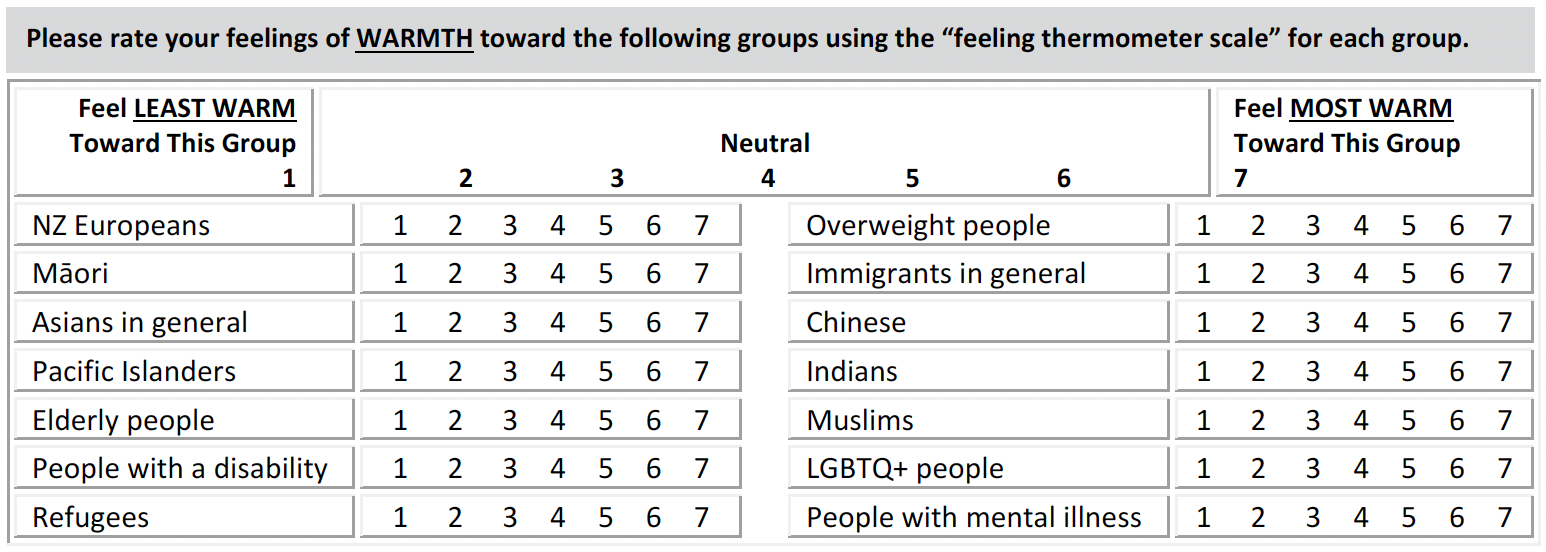
\includegraphics{figs/warmth.png}

}

\caption{\label{fig-warmth}Feeling thermometer scale}

\end{figure}%

\subsubsection{Felt belonging}\label{felt-belonging}

\begin{enumerate}
\def\labelenumi{\arabic{enumi}.}
\tightlist
\item
  I know that people in my life accept and value me. (1 = Very
  Innacurate, 7 = Very Accurate).
\item
  I feel like an outsider. (1 = Very Innacurate, 7 = Very Accurate).
\item
  I know that people in around me share my attitudes and beliefs. (1 =
  Very Innacurate, 7 = Very Accurate).
\end{enumerate}

\subsubsection{Support}\label{support}

\begin{enumerate}
\def\labelenumi{\arabic{enumi}.}
\tightlist
\item
  There are people I can depend on to help me if I really need it. (1 =
  Strongly Disagree, 7 = Strongly Agree).
\item
  There is no one I can turn to for guidance in times of stress (R). (1
  = Strongly Disagree, 7 = Strongly Agree).
\item
  I know there are people I can turn to when I need help. (1 = Strongly
  Disagree, 7 = Strongly Agree).
\end{enumerate}

\subsubsection{Employment}\label{employment}

\begin{enumerate}
\def\labelenumi{\arabic{enumi}.}
\tightlist
\item
  What is your highest level of qualification? (String entry).
\item
  Are you currently employed (This includes self-employed of casual
  work)? (Yes/No). This leads to a four-point nominal response: employed
  full-time, employed part-time, unemployed, and not in the labour
  force.
\item
  In that job, what is your current occupation? (String entry).
\item
  What is the main activity of the business or employer that you work
  for? (String entry).
\item
  How long have you worked at your current organization? (String entry:
  years/months).
\item
  How satisfied are you with your current job? (1 = Not Satisfied, 7 =
  Very Satisfied).
\item
  How secure do you feel in your current job? (1 = Not Secure, 7 = Very
  Secure).
\item
  How valued do you feel by your current organization? (1 = Not valued,
  7 = Very Valued).
\end{enumerate}

\subsubsection{Health}\label{health}

\begin{enumerate}
\def\labelenumi{\arabic{enumi}.}
\tightlist
\item
  In general, would you say your health is\ldots{} (1 = Poor, 7 =
  Excellent).
\item
  I seem to get sick a little easier than other people. (1 = Strongly
  Disagree, 7 = Strongly Agree).
\item
  I expect my health to get worse. (1 = Strongly Disagree, 7 = Strongly
  Agree).
\item
  Do you have a health condition or disability that limits you, and that
  has lasted for 6+ months? (Yes/No). If yes, please state: (String
  entry).
\item
  How often do you have a drink containing alcohol? This is measured
  using a 6 point nominal scale (a. Never - I don't drink, b. Monthly or
  less, c.~Up to 4 times a month, d.~Up to 3 times a week, e. 4 or more
  times a week, f.~Don't know).
\item
  Have you ever regularly smoked tobacco cigarettes? (Yes/No).
\item
  Have you ever regularly used e-cigarettes? (Yes/No).
\item
  Do you currently smoke tobacco cigarettes? (Yes/No).
\item
  Do you currently vape or use e-cigarettes? (Yes/No).
\item
  Access to and satisfaction with GP: Do you have a regular family
  doctor/GP? (Yes/No). (If yes) How satisfied are you with the service
  and care you receive from your family doctor/GP? (1 = Not Satisfied, 7
  = Very Satisfied). Do you think your doctor/GP shares a similar
  cultural background to you? (1 = Definitely No, 7 = Definitely Yes).
  Does your doctor/GP respect your cultural background when you are
  discussing health issues with them? (1= Definitely No, 7 = Definitely
  Yes).
\item
  Please estimate how many hours you spent during each of the following
  things last week (String entry). Options provided: Working in paid
  employment, housework/cooking, looking after children,
  volunteer/charitable work, exercising/physical activity, watching
  TV/Netflix/movies, travelling/commuting, watching/reading news, using
  the internet (in total), using social media (e.g., Facebook), playing
  video games/computer games.
\item
  BMI: Calculated by using a person's weight (Kg) divided by square root
  of height (m) that is asked separately, using ``What is your height?
  (String entry (meters))'', and ``What is your weight? (String entry
  (Kgs))''.
\item
  During the past month, on average, how many hours of actual sleep did
  you get per night? (String entry).
\item
  Do you have a health condition or disability that limits you, and that
  has lasted for 6+ months? (Yes/No). If yes, please state: (String
  entry).
\item
  Chronic diseases diagnosis: See Figure~\ref{fig-chrondis}.
\end{enumerate}

\begin{figure}

\centering{

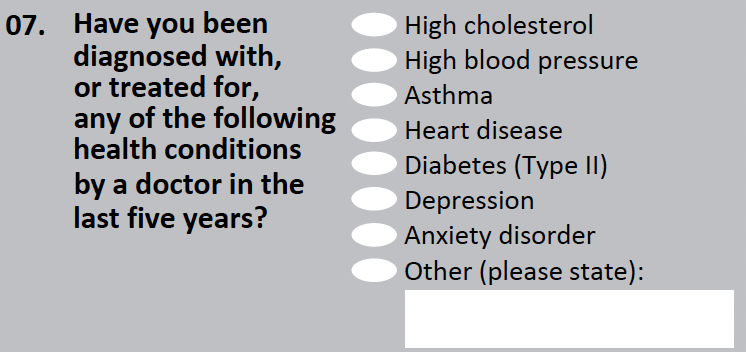
\includegraphics{figs/chronic-disease.png}

}

\caption{\label{fig-chrondis}Chronic disease diagnosis}

\end{figure}%

\subsubsection{Subjective wellbeing/psychological
distress}\label{subjective-wellbeingpsychological-distress}

Measured using the Kessler-6 items (items 1-6 in
Figure~\ref{fig-Kess-6}) rated on a 5-point scale (0 = None of the time,
4 = All of the time) (Kessler et al. 2010).

\begin{figure}

\centering{

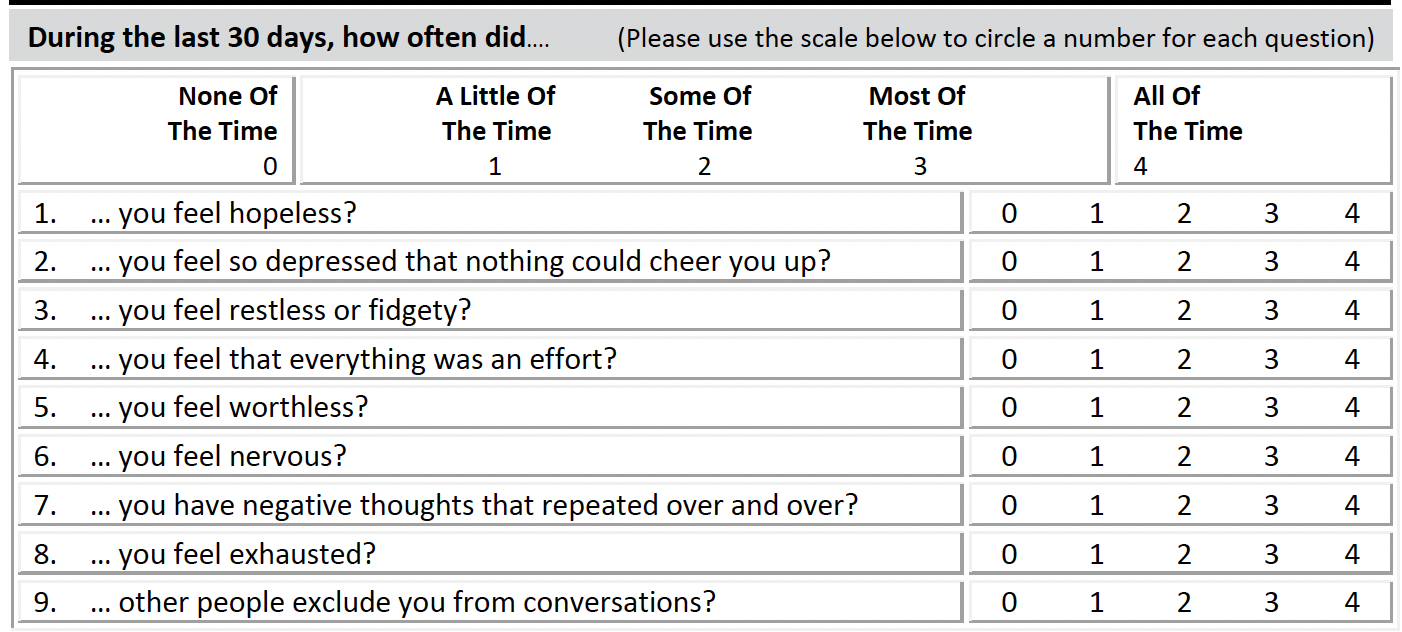
\includegraphics{figs/kessler-6.png}

}

\caption{\label{fig-Kess-6}Kessler-6 subjective wellbeing scale}

\end{figure}%

\subsubsection{Meaning of life}\label{meaning-of-life}

Items are: ``My life has a clear sense of purpose'' (1 = Strongly
Disagree, 7 = Strongly Agree) and ``I have a good sense of what makes my
life meaningful'' (1 = Strongly Disagree, 7 = Strongly Agree).

\subsubsection{Life satisfaction and national
wellbeing}\label{life-satisfaction-and-national-wellbeing}

Items from Figure~\ref{fig-life-sat} measured on 11-item measure (0 =
Completely Dissatisfied, 10 = Completely Satisfied). In addition, ``I am
satisfied with my life (1= Strongly Disagree, 7 = Strongly Agree)'' and
``In most ways my life is close to ideal (1 = Strongly Disagree, 7 =
Strongly Agree)'' are used.

\begin{figure}

\centering{

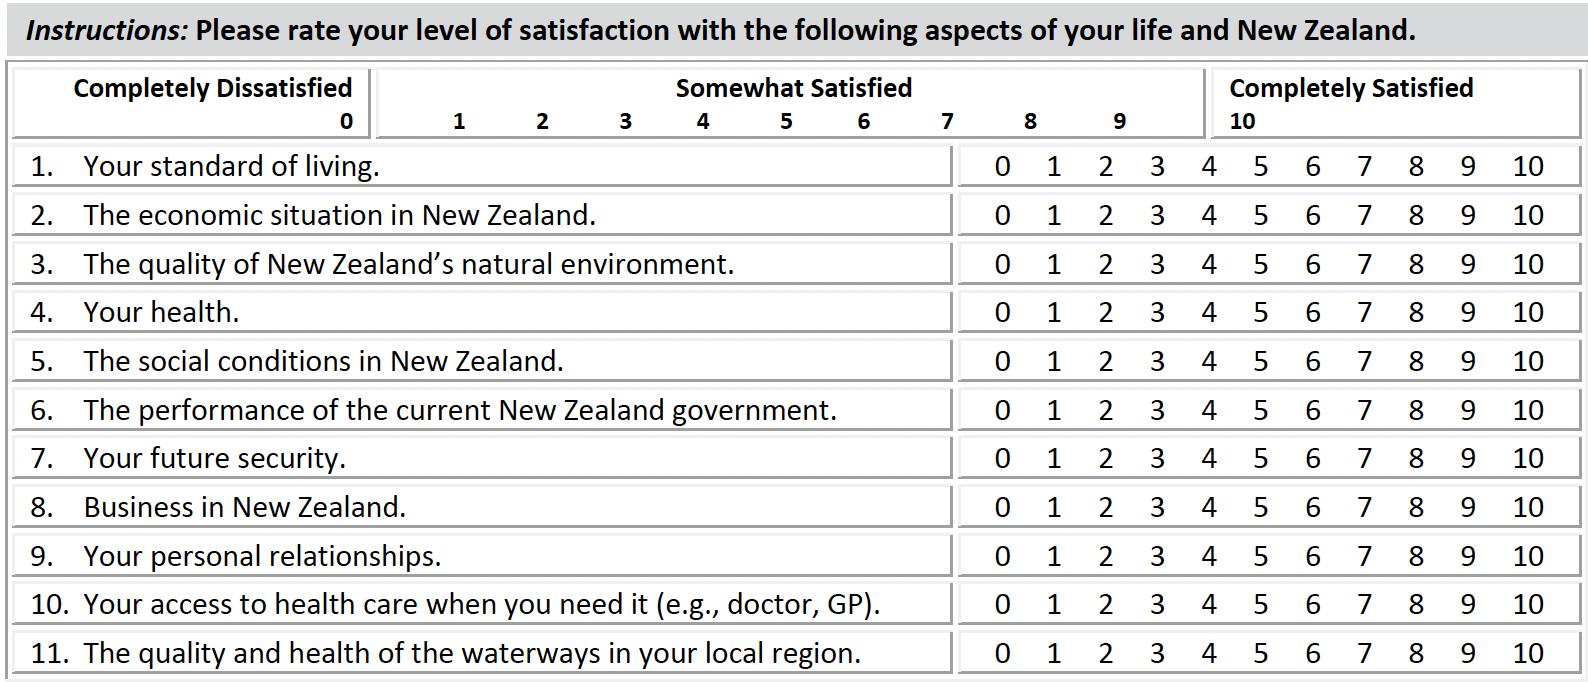
\includegraphics{figs/life-sat.png}

}

\caption{\label{fig-life-sat}Life Satisfaction scale}

\end{figure}%

\subsubsection{Self esteem}\label{self-esteem}

Items are, ``On the whole I am satisfied with myself''(1 = Very
Inaccurate, 7 = Very Accurate), ``I take a positive attitude toward
myself'' (1 = Very Inaccurate, 7 = Very Accurate) and ``I am inclined to
feel that I am a failure'' (R) (1 = Very Inaccurate, 7 = Very Accurate).

\subsubsection{Gratitude}\label{gratitude}

Items are, ``I have much in my life to be thankful for'' (1 = Strongly
Disagree, 7 = Strongly Agree), ``When I look at the world, I don't see
much to be grateful for'' (1 = Strongly Disagree, 7 = Strongly Agree)
and ``I am grateful to a wide variety of people'' (1 = Strongly
Disagree, 7 = Strongly Agree).

\subsubsection{Community making}\label{community-making}

I feel a sense of community with others in my local neighbourhood (1 =
Strongly Disagree, 7 = Strongly Agree).

\subsubsection{Intergroup anxiety}\label{intergroup-anxiety}

I feel anxious about interacting with people from other races (1 =
Strongly Disagree, 7 = Strongly Agree).

\subsubsection{Rumination}\label{rumination}

During the last 30 days, how often did you have negative thoughts that
repeated over and over? (0 = None of the time, 4 = All of the time).

\subsubsection{Forgivingness versus vengeful
rumination}\label{forgivingness-versus-vengeful-rumination}

Items are, ``Sometimes I can't sleep because of thinking about past
wrongs I have suffered.'' (1 = Strongly Disagree, 7 = Strongly Agree),
``I can usually forgive and forget when someone does me wrong. (R)'' (1
= Strongly Disagree, 7 = Strongly Agree), and ``I find myself regularly
thinking about past times that I have been wronged.'' (1 = Strongly
Disagree, 7 = Strongly Agree).

\subsubsection{Matching with other religious
groups}\label{matching-with-other-religious-groups}

Similar to Bulbulia et al. (2023), we will use the following variables
to identify matching members in different religions groups.

\begin{enumerate}
\def\labelenumi{\arabic{enumi}.}
\item
  Age: ``What is your age?'' (String entry), and ``When is your date of
  birth?'' (String entry).
\item
  Education: Measured by an 11-point ordinal scale (0 = No
  Qualification, 11 = Doctoral Degree, based on the New Zealand
  Qualification Framework ({``The New Zealand Qualifications
  Framework''} 2016)) from responses to the qualification-related
  question.
\item
  Employment: A binary variable is created (0 = Unemployed, 1 =
  Employed) based on the responses to employment item ``Are you
  currently employed?''.
\item
  Ethnicity: The items displayed in Figure~\ref{fig-ethnicgroups} are
  categorised following the New Zealand Census Groups: European, Māori,
  Pacific Peoples, Asian, MELAA (Middle Eastern, Latin
  American/African), and Other.
\item
  Gender: Responses to the string entry item ``What is your gender?''
  will be used to create a binary variable (Male = 1, Not male = 0).
\item
  Area-unit deprivation: Measured based on 2018 New Zealand Deprivation
  Index (Atkinson, Salmond, and Crampton 2019) that assigns a
  decile-rank index (1 = Least Deprived, 10 = Most Deprived) using
  participants' immediate neighbourhood's aggregate census information.
  This index is calculated using component factor analysis of nine
  variables in weighted order as follows: proportion of adults who
  received a means-tested benefit, household income, proportion not
  owning own home, proportion of single-parent families, the proportion
  of unemployed, proportion lacking qualifications, proportion household
  crowding, proportion no telephone access, and proportion no car
  access. Hence, this index reflects nationwide mean deprivation level
  for small neighbourhood-type units (i.e., small community areas
  consisting about 80-90 people).
\item
  Socioeconomic status (Occupational prestige): A census-derived
  occupation-based measure NZSEI (New Zealand Socioeconomic Index) is
  used to estimate one's socioeconomic status. It uses an open-ended
  question regarding one's occupation, which is subsequently classified
  in accordance with the Australian and New Zealand Standard
  Classification of Occupations (ANZSCO) Level 3. In the case of missing
  values, the measures is imputed using a combination of age and
  education. The measure is assigned scores between 10 = Low and High =
  90.
\item
  Parent: Measured by assigning a binary variable (1 = Those with
  children, 0 = The rest) to the item: ``How many children have you
  given birth to, fathered, or adopted?''. (String entry).
\item
  Partner: Responses to ``What is you relationship status?'' are
  assigned a binary variable (1 = Has a partner, 0 = Doesn't have a
  partner).
\item
  Religious identification: Responses to ``Do you identify with a
  religion and/or spiritual group?'' are coded a binary variable (1 =
  Yes, 0 = No).
\item
  Political orientation: Responses to ``Please rate how politically
  left-wing versus right-wing you see yourself as being'' are assigned a
  7-point scale (1 = Extremely left-wing, 7 = Extremely right-wing).
\item
  Residence: Urban or rural residence (a two-item nominal variable) is
  identified based on the physical addresses provided.
\item
  Region of habituation: Whether participants are living in an urban or
  rural area, based on the addresses provided, is coded; 1 = Urban, 0 =
  Rural.
\item
  Race-based rejection anxiety: ``People from other races would be
  likely to reject me on the basis of my race''. (1 = Strogly Disagree,
  7 = Strongly Agree).
\item
  Big Six personality traits: Six personality traits, agreeableness,
  conscientiousness, extraversion, openness, honesty-humility, and
  neuroticism, are measured using a 7-point (1 = Very Inaccurate, 7 =
  Very Accurate) Mini-IPIP6 scale (Sibley et al. 2011).
\end{enumerate}

\begin{figure}

\centering{

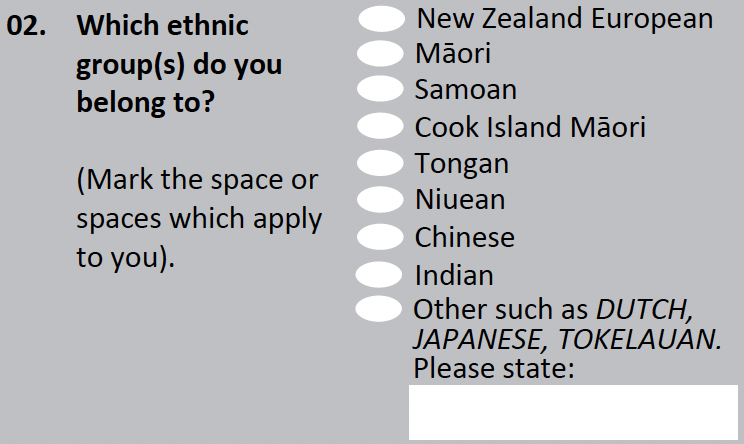
\includegraphics{figs/ethnic-groups.png}

}

\caption{\label{fig-ethnicgroups}Ethnic groups}

\end{figure}%

\subsection{Ethics}\label{ethics}

The NZAVS was approved by the University of Auckland Human Participants
Ethics Committee on 26 May 2021 until 26 May 2027 (Reference:
UAHPEC22576). All participants granted informed written consent and the
University of Auckland Human Participants Ethics Committee approved all
procedures.

\subsection{Design}\label{design}

MDS is a three-year-long booster for NZAVS. NZAVS is a planned
20-year-long longitudinal panel study of adult New Zealanders, currently
in its 15th year (Wave 15) that correponds with Wave 1 (the firs year)
of MDS (15 Oct 2023 to 14 Oct 2024). Wave 2 and Wave 3 of MDS will
correspond with NZAVS Wave 16 (15 Oct 2024 to 14 Oct 2025) and Wave 17
(15 Oct 2025 to 14 Oct 2026), respectively. NZAVS uses quantitative
measures. The following dependent variables will be considered to test
the proposed MDS hypotheses.

\begin{enumerate}
\def\labelenumi{\arabic{enumi}.}
\tightlist
\item
  Perceived religious discrimination
\item
  Perceived ethnic discrimination
\item
  Employment status
\item
  Job satisfaction
\item
  Job security
\item
  Feeling valued by organisation
\item
  Self-rated health
\item
  Perceived health decline
\item
  Chronic diseases and disabilities
\item
  Kessler-6 psychological distress scale
\item
  Meaning of life
\item
  Life satisfaction
\item
  Sense of belonging
\item
  Perceived support
\item
  Warmth toward various groups
\item
  Vengeful rumination
\item
  Forgiveness
\end{enumerate}

\subsection{Data Analysis}\label{data-analysis}

\subsubsection{Hypothesis 1}\label{hypothesis-1}

\begin{itemize}
\tightlist
\item
  Correlation between religiosity and prejudice
\item
  Regression: Service attendance, prayer frequency, religious
  importance, and spiritual identification (IVs) and perceived
  discrimination (DV)
\item
  Moderation: Testing whether or not community involvement moderates the
  relationship between religiosity and perceived discrimination.
\item
  Mediation: Whether or not the sense of belonging mediates relationship
  between religiosity and perceived discrimination.
\end{itemize}

\subsubsection{Hypothesis 2}\label{hypothesis-2}

\begin{itemize}
\tightlist
\item
  Using propensity score matching to match Muslims with participants
  from other religious groups based on variables used in previous
  publications, such as Bulbulia et al. (2023). These are: age,
  education, employment, ethnicity, gender, deprivation index,
  socioeconomic status, being a parent, having a partner, religious
  identification, political orientation, urban vs.~rural residence,
  region, race-based anxiety, and Big Six personality measures.
\item
  Regression: Employment status (binary) predicted from religious
  affiliation, job satisfaction, and job security.
\item
  Regression: Self-rated health and disability predicted from religious
  affiliation, health behaviours, and chronic diseases.
\item
  Chi square: Religious affiliation vs employment status and disability
  status.
\end{itemize}

\subsubsection{Hypothesis 3}\label{hypothesis-3}

\begin{itemize}
\tightlist
\item
  Matching participants similar to Hypothesis 2.
\item
  ANOVA: Comparing average scores of subjective wellbeing as well as
  psychological distress between Muslims and members of other religions.
\item
  Regression: Community support and religious community-making buffering
  against distress and enhancing wellbeing
\item
  Structural equation modelling: Modelling mediation of community-making
  on the relationship between religious affiliation and wellbeing
  outcomes.
\item
  Moderation: To find out whether the strength of community support and
  belonging moderate the effects of religious group membership on
  wellbeing and distress.
\end{itemize}

\subsection{Preregistration}\label{preregistration}

The hypotheses, measures, and proposed data analysis are preregistered
on OSF (\url{https://doi.org/10.17605/OSF.IO/B39XT}). The study was
preregistered before any attempted data analyses.

\subsection{Procedure}\label{procedure}

\subsubsection{Research assistant recruitment and
training}\label{research-assistant-recruitment-and-training}

The 30 research assistants, as indicated in
Table~\ref{tbl-muslim-population}, were recruited before the MDS Wave 1.
The position was advertised by University of Canterbury and shared via
social media, emails, and community organisations. The eligibility
criteria included the least of tertiary level education in New Zealand,
familiarity with research in humanities, interest in working with
community, and experiences of working with a Muslim community
organisation. Thirty research assistants were recruited after initial
screening and interviews from a total of 95 applicants.

Before the commencement of study, a series of comprehensive Zoom
trainings took place to familiarise research assistants with NZAVS, the
MDS background, and survey questionnaires. In addition, research
assistants learned about ethnical guidelines, confidentiality
principles, and interacting with a culturally diverse participants pool.

\subsubsection{Data collection}\label{data-collection}

Research assistants used the snowball approach for data collection. They
started reaching out to their close circles, and kept expanding their
reach. The sample was non-representative, and participants had the
choice of filling in the online questionnaire using Qualtrics, or a
paper questionnaire and returning it to the NZAVS headquarters in
Auckland University using a pre-paid postal envelope.

After the initial stage of reaching out to the close circle, the
research assistants started reaching out to community organisations. A
runsheet was provided, and different documents and promotional materials
such as individual messages, community messages, flyers, and posters
were at the research assistants disposal based on their needs. We have
also developed a clear vision statement and ethics statement that were
part of our MDS introductory letter. In addition, an additinal cover
letter was sent to all Muslim participants alongside the information
sheet. It was aimed to clearly convey the purposes of booster to the
community. Please see appendices A-H for these materials. Finally, 10
promotional shirts were designed that the research assistants wore
during festivals and community events for study promotion.

The social media campaign started at the beginning of 2024 and continued
until the end of Wave 1. Beside regular posts on a weekly, and later on,
on a fortnighly basis; we also used paid promotion to increase reach of
the project.

For the purposes of community promotion, we relied on a combination of
community outreach at local mosques, religious, community, and ethnic
organisations, Muslim schools and businesses, and MSA's (Muslim Student
Associations). From available databases and community contacts, we
identified 218 organisations and RAs were able to approach Muslims in
105 organisations. Out of these, 80 have endorsed and promoted the
study. Different organisations endorsed us in different manners: some
allowed us to give speeches to their audience, others shared our
promotional material online in social media, community message groups
(e.g., WhatsApp), and mailing lists. In addition, tens of posters were
placed in community facilities (e.g., mosques) and hundreds of flyers
were handed over after Friday prayers as well as cultural and religious
festivals.

In addition to reaching out to organisations, the principal investigator
conversed with 28 local and national community leaders, celebrities,
religious scholars, and academics to spread our message to the
communities. As part of this recruitment drive, the principal
investigator also presented 28 talks, presentations, or lectures to
Muslim community groups around New Zealand via mosques, universities, or
community organisations in the mentioned cities, explaining the goals of
the NZAVS, and how it would benefit the New Zealand Muslim community to
be represented in this ongoing national longitudinal panel sample. Five
additional talks were delivered by research assistants too.

\subsubsection{Ensuring research assistants'
convenience}\label{ensuring-research-assistants-convenience}

MDS research assistants come from differnet backgrounds. Some of them
have had extensive researcch experience, whereas, for the some of them,
it was the first attempt of engaging in data collection. Some research
assistants wanted explicit weekly targets and others decided their own
targets. The principal investigator conducted fortnightly check-ins with
individuals and teams in cities to ensure that questions are answered,
and was always available to guide the process, provide feedback. The
principal investigator was also available talk with participants if and
when needed via audio and video mediums.

\subsubsection{Web hosting}\label{web-hosting}

The MDS website (access from
\href{https://linktr.ee/muslimdiversity}{here}) provides the most
up-to-date and needed information for public and professionals and will
keep updating as we make progress.

\subsubsection{Data management}\label{data-management}

The collected data are processed in the NZAVS headquarters,
deidentified, and only made available to trusted researchers and
collaborators. The NZAVS data dictionary, sampling procedure, sample
details and other relevant information can be accessed online
(\url{https://osf.io/75snb/wiki/home/}) (Sibley 2024).

\subsection{Timeline}\label{timeline}

\begin{figure}

\centering{

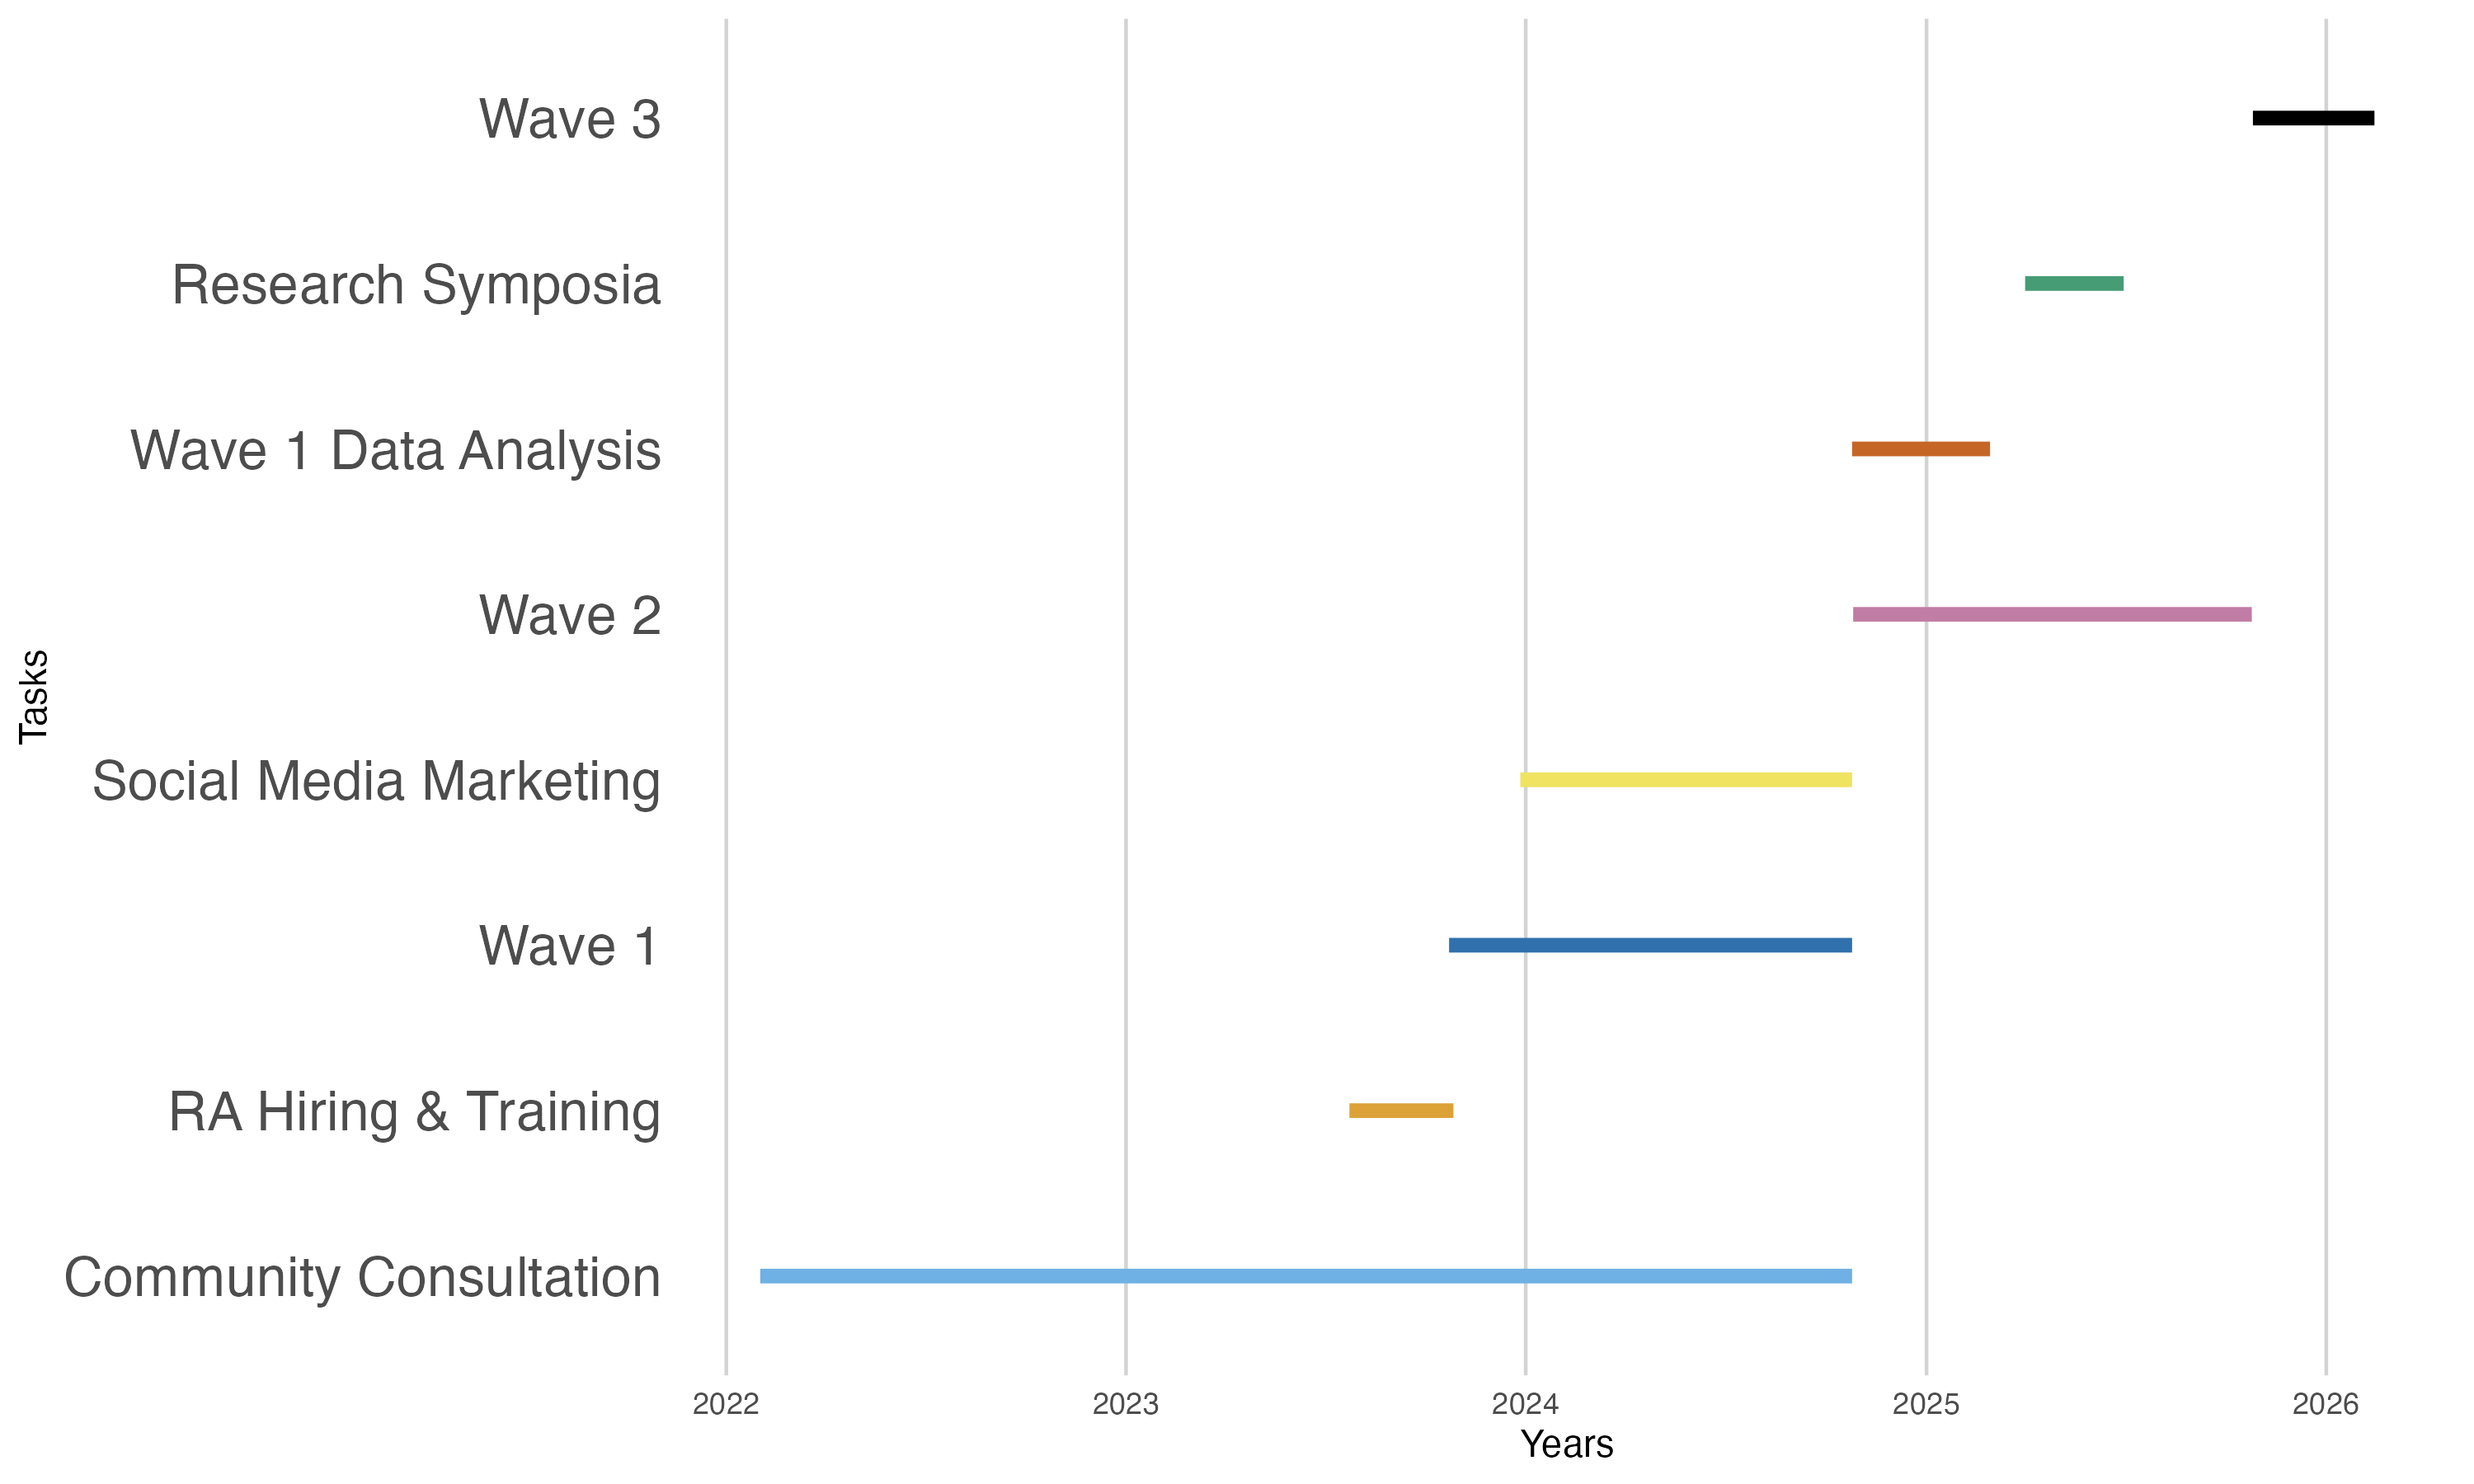
\includegraphics{figs/project_timeline.png}

}

\caption{\label{fig-timeline}MDS timeline showing tasks and durations}

\end{figure}%

As displayed in Figure~\ref{fig-timeline}, the community consultation
started before Wave 1 and continued until the end of it. In addition,
social media marketing has been an integral part of MDS data collection
campaign. The planned future events, with approximate dates, are
indicated too.

\subsection{Enablers and challengers of data
collection}\label{enablers-and-challengers-of-data-collection}

Based on our interactions with the Muslim community and feedback from
research assistants, we anecdotally know that the following elements
encourage increased participantion of the Muslim community in research.

\begin{enumerate}
\def\labelenumi{\arabic{enumi}.}
\tightlist
\item
  Building rapport
\item
  Addressing concerns regarding confidentiality and data management
\item
  Being transparent and truthful with the community
\item
  Approaching the community via trusted leaders
\item
  Reaching out to inviduals personally, not via groups.
\end{enumerate}

We also learned that the following factors could hinder data collection
efforts.

\begin{enumerate}
\def\labelenumi{\arabic{enumi}.}
\tightlist
\item
  Length of the questionnaire measured by the time taken to complete it
\item
  Unfamiliarity of participants with scientific research
\item
  Privacy concerns
\item
  Political climate
\item
  Language barriers
\item
  Generatioanl differences, with older generations less likely to take
  part.
\end{enumerate}

Although these findings are anecdotal, we have witnessed enhanced
participation by addressing some of the challengers to data collection.
To better understand and document, we have conducted a qualitative
research of research assistant experiences in terms of data collection
(Badis and Afzali 2024). Findings from this research will be published
in the near future.

\subsection{Strengths and limitations}\label{strengths-and-limitations}

Quantitative only. focus on english speakers only 1. Zahra E, Rizwan,
Somia

Generalisablity

Mentions Jamila's and Qual here..

\subsection{Application and
implications}\label{application-and-implications}

Aamina Ali, Adepate Mustapha-Koiki

Potential contributions of the study to the field of mental health
research and implications for policy and practice.

\subsection{Conclusion}\label{conclusion}

MDS is a crucial booster for the NZAVS because not only it addresses the
under-representation of Muslim in NZVAS, but it only helps us answer
many questions about Muslims' self-perception, meaning-making,
flourishing, religiosity, and health outcomes. The current protocol also
provides a preliminary understanding of how to work with a minoritised
religious community in a culturally sensitive manner. Further
discoveries are going to be published by the MDS team in the near
future. Despite the well-known limitations of observational,
quantitative, survey research, MDS provides substantial values in terms
of implications and applications. Techniques learned from MDS can be
applied while working with Muslims and other culturally similar groups
in New Zealand and overseas.

\newpage{}

\section*{References}\label{references}
\addcontentsline{toc}{section}{References}

\phantomsection\label{refs}
\begin{CSLReferences}{1}{0}
\bibitem[\citeproctext]{ref-arkilic2020}
Arkilic, Ayca. 2020. {``What Is {I}slam's Appeal to {M}{ā}ori?''}
\url{http://newsroom.co.nz/2020/08/18/what-is-islams-appeal-to-maori/}.

\bibitem[\citeproctext]{ref-arkilic2021a}
---------. 2021. {``The {C}hristchurch Shooting and the 2020 {N}ew
{Z}ealand Election.''} In, edited by Stephen Levine, 225--39.
Wellington, New Zealand: Victoria University Press.

\bibitem[\citeproctext]{ref-atkinson2019}
Atkinson, June, Clare Salmond, and Peter Crampton. 2019. {``NZDep2018
Index of Deprivation.''}

\bibitem[\citeproctext]{ref-badis2024}
Badis, Jamila Shirley, and Usman Afzali. 2024. {``Enablers and
Challengers of Collecting Data from Muslim Community in Aotearoa New
Zealand.''} \emph{OSF}. \url{https://doi.org/10.17605/OSF.IO/8F36H}.

\bibitem[\citeproctext]{ref-barger2010}
Barger, Brian, Robin Nabi, and Liang Yu Hong. 2010. {``Standard
Back-Translation Procedures May Not Capture Proper Emotion Concepts: A
Case Study of Chinese Disgust Terms.''} \emph{Emotion} 10 (5): 703--11.
\url{https://doi.org/10.1037/a0021453}.

\bibitem[\citeproctext]{ref-bulbulia2023}
Bulbulia, Joseph A, M Usman Afzali, Kumar Yogeeswaran, and Chris G
Sibley. 2023. {``Long-Term Causal Effects of Far-Right Terrorism in New
Zealand.''} Edited by M Gelfand. \emph{PNAS Nexus} 2 (8).
\url{https://doi.org/10.1093/pnasnexus/pgad242}.

\bibitem[\citeproctext]{ref-byrne2022}
Byrne, Kate G., Kumar Yogeeswaran, Martin J. Dorahy, Jessica Gale, M.
Usman Afzali, Joseph Bulbulia, and Chris G. Sibley. 2022.
{``Psychological Impact of Far-Right Terrorism Against Muslim Minorities
on National Distress, Community, and Wellbeing.''} \emph{Scientific
Reports} 12 (1): 1620. \url{https://doi.org/10.1038/s41598-022-05678-x}.

\bibitem[\citeproctext]{ref-drury2016}
Drury, A. 2016. {``{Islam{'}s} History and Integration in the {N}ew
{Z}ealand Society: A {Convert{'}s} View.''} In, edited by E Kolig and
Voyce M, 113--29. Maryland, USA: Rowman.

\bibitem[\citeproctext]{ref-fenn2020}
Fenn, Jessy, Chee-Seng Tan, and Sanju George. 2020. {``Development,
Validation and Translation of Psychological Tests.''} \emph{BJPsych
Advances} 26 (5): 306--15. \url{https://doi.org/10.1192/bja.2020.33}.

\bibitem[\citeproctext]{ref-frykberg2023}
Frykberg, Laura. 2023. {``Online Hate Towards Muslims 'Increasing' Since
Mosque Attacks.''}
\url{https://www.1news.co.nz/2023/03/12/online-hate-towards-muslims-increasing-since-mosque-attacks/}.

\bibitem[\citeproctext]{ref-greaves2020}
Greaves, Lara M., Aarif Rasheed, Stephanie D'Souza, Nichola Shackleton,
Luke D. Oldfield, Chris G. Sibley, Barry Milne, and Joseph Bulbulia.
2020. {``Comparative Study of Attitudes to Religious Groups in New
Zealand Reveals Muslim-Specific Prejudice.''} \emph{K{ō}tuitui: New
Zealand Journal of Social Sciences Online} 15 (2): 260--79.
\url{https://doi.org/10.1080/1177083x.2020.1733032}.

\bibitem[\citeproctext]{ref-hawi2019}
Hawi, Diala, Danny Osborne, Joseph Bulbulia, and Chris G. Sibley. 2019.
{``Terrorism Anxiety and Attitudes Toward Muslims.''} \emph{New Zealand
Journal of Psychology} 48 (1): 8089.

\bibitem[\citeproctext]{ref-islamoph2022}
{``Islamophobia After {C}hristchurch Terror Attacks Quadrupled -
{A}ustralian Report.''} 2022.
\url{https://www.rnz.co.nz/news/national/463304/islamophobia-after-christchurch-terror-attacks-quadrupled-australian-report}.

\bibitem[\citeproctext]{ref-jacinda2019b}
{``Jacinda {A}rdern on the {C}hristchurch Shooting: 'One of {N}ew
{Z}ealand's Darkest Days'.''} 2019.
\url{https://www.theguardian.com/world/2019/mar/15/one-of-new-zealands-darkest-days-jacinda-ardern-responds-to-christchurch-shooting}.

\bibitem[\citeproctext]{ref-junaid2024}
Junaid, Fatima A., S. Cassim, and J. Khan-Janif. 2024. {``Muslims'
Experiences of Inclusion, Discrimination, {I}slamophobia and Wellbeing
in {A}otearoa {N}ew {Z}ealand.''}
\url{https://doi.org/10.13140/RG.2.2.12693.74725/1}.

\bibitem[\citeproctext]{ref-kabir2024}
Kabir, Shah Nister. 2024. {``{`}They Are Us{'}: Orientalist Perspective
Challenged in New Zealand Newspapers{'} Coverage.''} \emph{Journal of
Arab \& Muslim Media Research}, January.
\url{https://doi.org/10.1386/jammr_00077_1}.

\bibitem[\citeproctext]{ref-kessler2010}
Kessler, Ronald C., Jennifer Greif Green, Michael J. Gruber, Nancy A.
Sampson, Evelyn Bromet, Marius Cuitan, Toshi A. Furukawa, et al. 2010.
{``Screening for Serious Mental Illness in the General Population with
the K6 Screening Scale: Results from the WHO World Mental Health (WMH)
Survey Initiative.''} \emph{International Journal of Methods in
Psychiatric Research} 19 (S1): 4--22.
\url{https://doi.org/10.1002/mpr.310}.

\bibitem[\citeproctext]{ref-ozolins2020}
Ozolins, Uldis, Sandra Hale, Xiang Cheng, Amelia Hyatt, and Penelope
Schofield. 2020. {``Translation and Back-Translation Methodology in
Health Research {\textendash} a Critique.''} \emph{Expert Review of
Pharmacoeconomics \& Outcomes Research} 20 (1): 69--77.
\url{https://doi.org/10.1080/14737167.2020.1734453}.

\bibitem[\citeproctext]{ref-rahman2019}
Rahman, Anjum. 2019. {``Islamic {W}omen's {C}ouncil Repeatedly Lobbied
to Stem Discrimination.''}
\url{https://www.rnz.co.nz/news/on-the-inside/384911/islamic-women-s-council-repeatedly-lobbied-to-stem-discrimination}.

\bibitem[\citeproctext]{ref-rahman2020}
Rahman, Khairiah A. 2020. {``News Media and the Muslim Identity After
the Christchurch Mosque Massacres.''} \emph{K{ō}tuitui: New Zealand
Journal of Social Sciences Online} 15 (2): 360--84.
\url{https://doi.org/10.1080/1177083x.2020.1747503}.

\bibitem[\citeproctext]{ref-raissi2024}
Raissi, Hussain. 2024. {``Exploring Senses of Belonging: {A}
Multidimensional Study of {M}uslim Immigrant Youth in {N}ew
{Z}ealand.''} PhD thesis, Dunedin.

\bibitem[\citeproctext]{ref-royalco2020}
{``Royal {C}ommission of {I}nquiry into the Terrorist Attack on
{C}hristchurch {M}asjidain on 15 {M}arch 2019.''} 2020.
\url{https://christchurchattack.royalcommission.nz}.

\bibitem[\citeproctext]{ref-shanaah2021}
Shanaah, Sadi, Kumar Yogeeswaran, Lara Greaves, Joseph A. Bulbulia,
Danny Osborne, M. Usman Afzali, and Chris G. Sibley. 2021. {``Hate
Begets Warmth? The Impact of an Anti-{M}uslim Terrorist Attack on Public
Attitudes Toward {M}uslims.''} \emph{Terrorism and Political Violence},
119.

\bibitem[\citeproctext]{ref-shaver2017}
Shaver, John H., Chris G. Sibley, Danny Osborne, and Joseph Bulbulia.
2017. {``News Exposure Predicts Anti-Muslim Prejudice.''} Edited by
Michiel van Elk. \emph{PLoS One} 12 (3): e0174606.
\url{https://doi.org/10.1371/journal.pone.0174606}.

\bibitem[\citeproctext]{ref-sibley2024}
Sibley, Chris G. 2024. {``New Zealand Attitudes and Values Study.''}
\url{https://osf.io/75snb/wiki/home/}.

\bibitem[\citeproctext]{ref-sibley2020}
Sibley, Chris G., M. Usman Afzali, Nicole Satherley, Anastasia Ejova,
Samantha Stronge, Kumar Yogeeswaran, Michael Grimshaw, Diala Hawi, Zahra
Mirnajafi, and Fiona Kate Barlow. 2020. {``Prejudice Toward {M}uslims in
{N}ew {Z}ealand: Insights from the {N}ew {Z}ealand {A}ttitudes and
{V}alues {S}tudy.''} \emph{New Zealand Journal of Psychology} 49 (1).

\bibitem[\citeproctext]{ref-sibley2011}
Sibley, Chris G., N. Luyten, Missy Purnomo, A. Mobberley, L. W. Wootton,
Matthew Hammond, Nikhil Sengupta, et al. 2011. {``The Mini-IPIP6:
Validation and Extension of a Short Measure of the {B}ig-{S}ix Factors
of Personality in {N}ew {Z}ealand.''} \emph{New Zealand Journal of
Psychology} 40 (3): 142--59.

\bibitem[\citeproctext]{ref-statsnz2024}
{``Stats NZ.''} 2024. \url{https://www.stats.govt.nz/}.

\bibitem[\citeproctext]{ref-sulaiman-hill2024}
Sulaiman-Hill, Ruqayya C., Richard Porter, Philip Schluter, Ben
Beaglehole, Shaystah Dean, Sandila Tanveer, Joseph Boden, and Caroline
Bell. 2024. {``Research Following Trauma in Minority Ethnic and Faith
Communities: Lessons from a Study of the Psychosocial Sequelae of the
Christchurch Mosque Terror Attacks.''} \emph{BJPsych Open} 10 (1).
\url{https://doi.org/10.1192/bjo.2023.641}.

\bibitem[\citeproctext]{ref-sulaiman-hill2021}
Sulaiman-Hill, Ruqayya C., Richard Porter, Sandila Tanveer, Joseph
Boden, Ben Beaglehole, Philip J. Schluter, Shaystah Dean, and Caroline
Bell. 2021. {``Psychosocial Impacts on the {C}hristchurch {M}uslim
Community Following the 15 March Terrorist Attacks: A Mixed-Methods
Study Protocol.''} \emph{BMJ Open} 11 (10): e055413.

\bibitem[\citeproctext]{ref-thenew2016}
{``The New Zealand Qualifications Framework.''} 2016.

\bibitem[\citeproctext]{ref-wilson2020}
Wilson, Chris, and Sanjal Shastri. 2020. {``Hate Crimes Against
{M}uslims Spiked After the Mosque Attacks, and {A}rdern Promises to Make
Such Abuse Illegal.''}
\url{http://theconversation.com/hate-crimes-against-muslims-spiked-after-the-mosque-attacks-and-ardern-promises-to-make-such-abuse-illegal-147347}.

\bibitem[\citeproctext]{ref-worldle2019}
{``World Leaders Condemn New Zealand Mosque Attacks.''} 2019.
\url{https://www.aljazeera.com/news/2019/3/15/the-world-reacts-to-new-zealand-mosque-attacks}.

\bibitem[\citeproctext]{ref-yogeeswaran2019}
Yogeeswaran, Kumar, M Usman Afzali, Nadia P Andrews, Elizabeth A
Chivers, Meng-Jie Wang, Thierry Devos, and Chris G Sibley. 2019.
{``Exploring {N}ew {Z}ealand National Identity and Its Importance for
Attitudes Toward {M}uslims and Support for Diversity.''} \emph{New
Zealand Journal of Psychology} 48 (1): 29--35.

\end{CSLReferences}

\newpage{}

\section{Study Registration}\label{study-registration}

This hypotheses and data analysis plan for this study were preregistred
at OSF \url{https://doi.org/10.17605/OSF.IO/B39XT}.

\section{Data Sharing}\label{data-sharing}

The data described in this study are part of the Muslim Diversity Study,
that is conducted under the \href{https://osf.io/75snb/}{New Zealand
Attitudes and Values Study}.

\section{Conflict of Interest}\label{conflict-of-interest}

The authors have no conflict of interest to disclose.

\section{Financial Support}\label{financial-support}

The Muslim Diversity Study - officially known as ``A National
Longitudinal Study of Muslim Diversity and Flourishing'' is supported by
a grant from the Templeton Religion Trust (TRT-2022-30579). The funders
had no role in preparing the manuscript or the decision to publish it.

\section{Acknoledgement/Gratitude:}\label{acknoledgementgratitude}

The authors are grateful to W. Joel Schneider for the
\href{https://github.com/wjschne/apaquarto}{Quarto template}.

\newpage{}

\section{CRediT Taxonomy Statement}\label{credit-taxonomy-statement}

\textbf{M. Usman Afzali:} Conceptualization, Data Curation, Formal
Analysis, Funding Acquisition, Investigation, Methodology, Project
Administration,Resources, Supervision, Visualization, Writing - Original
Draft, Writing - Review \& Editing. \textbf{Jamila Badis:} Data
Curation, Project Administration, Writing - Original Draft, Writing -
Review \& Editing. \textbf{Parus Khoso:} Data Curation, Formal analysis,
Writing - Original Draft (Pilot Community Consultation), Writing -
Review \& Editing. \textbf{Farah Shawkat:} Data Curation, Writing -
Original Draft (Method), Writing - Review \& Editing. \textbf{Fatima A.
Junaid:} Writing - Original Draft (Introduction), Writing - Review \&
Editing. \textbf{Ayca Arkilic:} Writing - Original Draft (Introduction),
Writing - Review \& Editing. \textbf{Mazharuddin Syed Ahmed:} Data
Curation, Writing - Review \& Editing \textbf{Hussain Raissi:} Data
Curation, Writing - Original Draft (Method), Writing - Review \&
Editing. \textbf{Hala Burhoum:} Data Curation, Writing - Original Draft
(Method), Writing - Review \& Editing. \textbf{Tuba Azeem:} Data
Curation, Writing - Original Draft (Method), Writing - Review \&
Editing. \textbf{Iman Husain:} Data Curation, Writing - Original Draft
(Method), Writing - Review \& Editing. \textbf{Zarqa Shaheen Ali:} Data
Curation, Writing - Original Draft (Method), Writing - Review \&
Editing. \textbf{Zahra Haidary:} Data Curation, Writing - Original Draft
(Method), Writing - Review \& Editing. \textbf{Mashal Khan:} Data
Curation, Writing - Original Draft (Method), Writing - Review \&
Editing. \textbf{Nasratullah Hamid:} Data Curation, Writing - Original
Draft (Method), Writing - Review \& Editing. \textbf{Gul e Aqsa:} Data
Curation, Writing - Review \& Editing. \textbf{Zahra Emamzadeh:} Writing
- Original Draft (Strengths and Limitations, Conclusion), Writing -
Review \& Editing. \textbf{Rizwan Sulehry:} Writing - Original Draft
(Strengths \& Limitations), Writing - Review \& Editing. \textbf{Somia
Tasneem:} Writing - Original Draft (Strengths and Limitations,
Conclusion), Writing - Review \& Editing. \textbf{Aamina Ali} Writing -
Original Draft (Applications \& Implications), Writing - Review \&
Editing. \textbf{Adepate Mustapha-Koiki:} Writing - original draft
(Applications \& Implications), Writing - Review \& Editing
\textbf{Afrah Ali Nadukkudi Puthenpura:} Writing - Review \& Editing
\textbf{Sandila Tanveer:} Writing - Review \& Editing \textbf{Aarif
Rasheed:} Conceptualization, Data Curation, Funding Acquisition,
Resources, Writing - Review \& Editing. \textbf{Kumar Yogeeswaran:}
Conceptualization, Funding Acquisition, Methodology, Writing - Original
Draft, Writing - Review \& Editing. \textbf{Chris G. Sibley:}
Conceptualization, Data Curation, Funding Acquisition, Methodology,
Project Administration,Resources, Supervision, Writing - Review \&
Editing, Development \& Management of the New Zealand Attitudes and
Values Study Panel Data Collection from 2009 to the Present.
\textbf{Joseph A. Bulbulia:} Conceptualization, Funding Acquisition,
Methodology, Project Administration, Resources, Supervision, Writing -
Original Draft, Writing - Review \& Editing.

\newpage{}

\section{Appendix A}\label{appendix-a}

\subsection{MDS Runhseet}\label{mds-runhseet}

{[}\texttt{Monospaced} font refers to urls in the actual document.{]}

\noindent Salam alaikum and welcome to the Muslim Diversity Study.

\begin{enumerate}
\def\labelenumi{\arabic{enumi}.}
\tightlist
\item
  This \texttt{Dropbox\ folder} consists of all information that you
  might need.
\item
  We have updated our communication and approach strategy, found
  \texttt{here}.
\item
  This \texttt{document} contains message to the community and FAQs.
  {[}will keep updating{]}
\item
  \texttt{Cover\ letter} for the Muslim Diversity Study.
\item
  MDS \texttt{Questionnaire} (pdf)
\item
  Use this \texttt{message} to send the MDS participation request to
  individuals. Please remember that individual connection is extremely
  important, and this is what we bank on.
\item
  Use this \texttt{message} to advertise MDS on social media (e.g.,
  Facebook or LinkedIn); and to send it via WhatsApp or emailing lists
  to the wider community and organizations.
\item
  Use this \texttt{message} for shorter social media platforms (e.g.,
  Twitter/X).
\item
  Access the \texttt{poster} (pdf) here (and png).
\item
  Access the \texttt{flyer} (pdf) here (and png).
\item
  This \texttt{document} can be shared with organizations to introduce
  MDS.
\item
  Organisation lists: \texttt{Auckland}, \texttt{Hamilton},
  \texttt{Palmerston\ North}, \texttt{Wellington},
  \texttt{Christchurch}, \texttt{Dunedin}. In addition, \texttt{this} is
  the list of organisations that have endorsed us or shared our ads.
  Please keep adding names to this list.
\item
  Please use \texttt{this} guideline for reaching out to organizations.
\item
  This \texttt{story} by UC has recorded the motivation behind MDS and
  its benefits for the Muslim community. It can be shared widely with
  those that want to know more.
\item
  The recent public \texttt{lecture} narrates the whole story of MDS
  (past, present, future) in a detailed manner. This, again, can be
  shared extensively with anyone interested.
\item
  Find our social media and website \texttt{here}.
\item
  The paper questionnaires are valuable, and to ensure meaningful
  responses, we shall only provide them to individuals who express
  interest and want them. Please distribute as many copies of
  \texttt{flyers}, and I can provide more flyers as needed.
\item
  Participants using the Qualtrics link should be reminded that they can
  resume the questionnaire from where they left off if they don't
  complete it initially. Ideally, an additional message can be sent
  using this wording: ``You can easily resume the questionnaire where
  you left off by clicking on the provided link. Feel free to complete
  the questionnaire in multiple sessions; your previous responses are
  automatically saved.'' Since it's not part of the ethics approval, it
  can be sent in the next message as additional guideline (instruction).
\item
  To claim your hours, log-in \texttt{here}.
\item
  If you are claiming your hours for the first time, use information in
  this \texttt{folder}.
\item
  If you want to have an update on collected data so far, see
  \texttt{this}.
\item
  I am thinking of a qualitative research project based on our
  experiences with the Muslim community where we'd want to interview our
  current RA's. It's briefly detailed \texttt{here}. If any of you are
  keen to be part of this or know someone who might want to take this
  on, please let me know. It can easily be a master's thesis, and as
  detailed in the brief, it will attract great impact.
\item
  \url{https://linktr.ee/muslims_nz}
\item
  \url{https://linktr.ee/muslimdiversity}
\end{enumerate}

\newpage{}

\section{Appendix B}\label{appendix-b}

\subsection{Message to Individual
Participnats}\label{message-to-individual-participnats}

Your Voice Matters! Join the Muslim Diversity Study!

\noindent Assalamu Alaikum WR WB {[}person's name{]}

\noindent I'm {[}name of the RA{]}, a research assistant in the Muslim
Diversity Study.

\noindent We need YOUR perspective!

\noindent The Muslim community is underrepresented, and we're changing
that with your help. Participate in this first-of-its-kind survey to
share your views on social attitudes, values, resilience, religiosity,
flourishing, meaning-making, wellbeing, and experiences of Muslims in
New Zealand. Let's make our voices heard!

\noindent Why Participate?

\noindent Gather data on underrepresented Muslims, amplifying voices and
providing insights into issues, wellbeing, and experiences.

\noindent Equip the Muslim community with evidence-based information for
advocacy.

\noindent Enrich understanding, strengthening the collective voice, and
shaping a more accurate narrative.

\noindent Your contribution counts and confidentially is assured!

\noindent By participating, you could potentially win one out of five
\$1000 grocery vouchers.

\noindent The data will be analysed with a focus on the Muslim
community. Your input guides our research, ensuring authenticity and
representation. We reassure you that the responses to the questionnaire
are anonymized, encrypted, and aggregated in a manner that ensure
confidentiality.

\noindent Spread the Word!

\noindent Please share with your friends, family, and community members!
Let's come together and make a difference.

\noindent To complete the questionnaire kindly click on the link below
or message us for a paper copy:
\url{https://www.nzavs.auckland.ac.nz/muslim_diversity}

\noindent For more info, visit our website (below) or reach out to Dr
Usman Afzali (the lead researcher): (email address and contact phone
number)
\url{https://www.canterbury.ac.nz/science/schools/psyc-speech-hear/research/muslim-diversity/}

\noindent APPROVED BY THE UNIVERSITY OF AUCKLAND HUMAN PARTICIPANTS
ETHICS COMMITTEE ON 26/05/2021 UNTIL 26/05/2027, REFERENCE NUMBER:
UAHPEC22576.

\newpage{}

\section{Appendix C}\label{appendix-c}

\subsection{Community and Social Media
Message}\label{community-and-social-media-message}

Your Voice Matters! Join the Muslim Diversity Study!

\noindent Assalamu Alaikum WR WB, Muslims in New Zealand!

\noindent We need YOUR perspective!

\noindent The Muslim community is underrepresented, and we're changing
that with your help. Participate in this first-of-its-kind survey to
share your views on social attitudes, values, resilience, religiosity,
flourishing, meaning-making, wellbeing, and experiences of Muslims in
New Zealand. Let's make our voices heard!

\noindent Why Participate?

\noindent Gather data on underrepresented Muslims, amplifying voices and
providing insights into issues, wellbeing, and experiences.

\noindent Equip the Muslim community with evidence-based information for
advocacy.

\noindent Enrich understanding, strengthening the collective voice, and
shaping a more accurate narrative.

\noindent Your contribution counts and confidentially is assured!

\noindent By participating, you could potentially win one out of five
\$1000 grocery vouchers.

\noindent The data will be analysed with a focus on the Muslim
community. Your input guides our research, ensuring authenticity and
representation. We reassure you that the responses to the questionnaire
are anonymized, encrypted, and aggregated in a manner that ensure
confidentiality.

\noindent Spread the Word!

\noindent Please share with your friends, family, and community members!
Let's come together and make a difference.

\noindent To complete the questionnaire kindly click on the link below
or message us for a paper copy:
\url{https://www.nzavs.auckland.ac.nz/muslim_diversity}

\noindent For more info, visit our website (below) or reach out to Dr
Usman Afzali (the lead researcher): (email address and contact phone
number)
\url{https://www.canterbury.ac.nz/science/schools/psyc-speech-hear/research/muslim-diversity/}

\noindent APPROVED BY THE UNIVERSITY OF AUCKLAND HUMAN PARTICIPANTS
ETHICS COMMITTEE ON 26/05/2021 UNTIL 26/05/2027, REFERENCE NUMBER:
UAHPEC22576.

\newpage{}

\section{Appendix D}\label{appendix-d}

\begin{figure}

\centering{

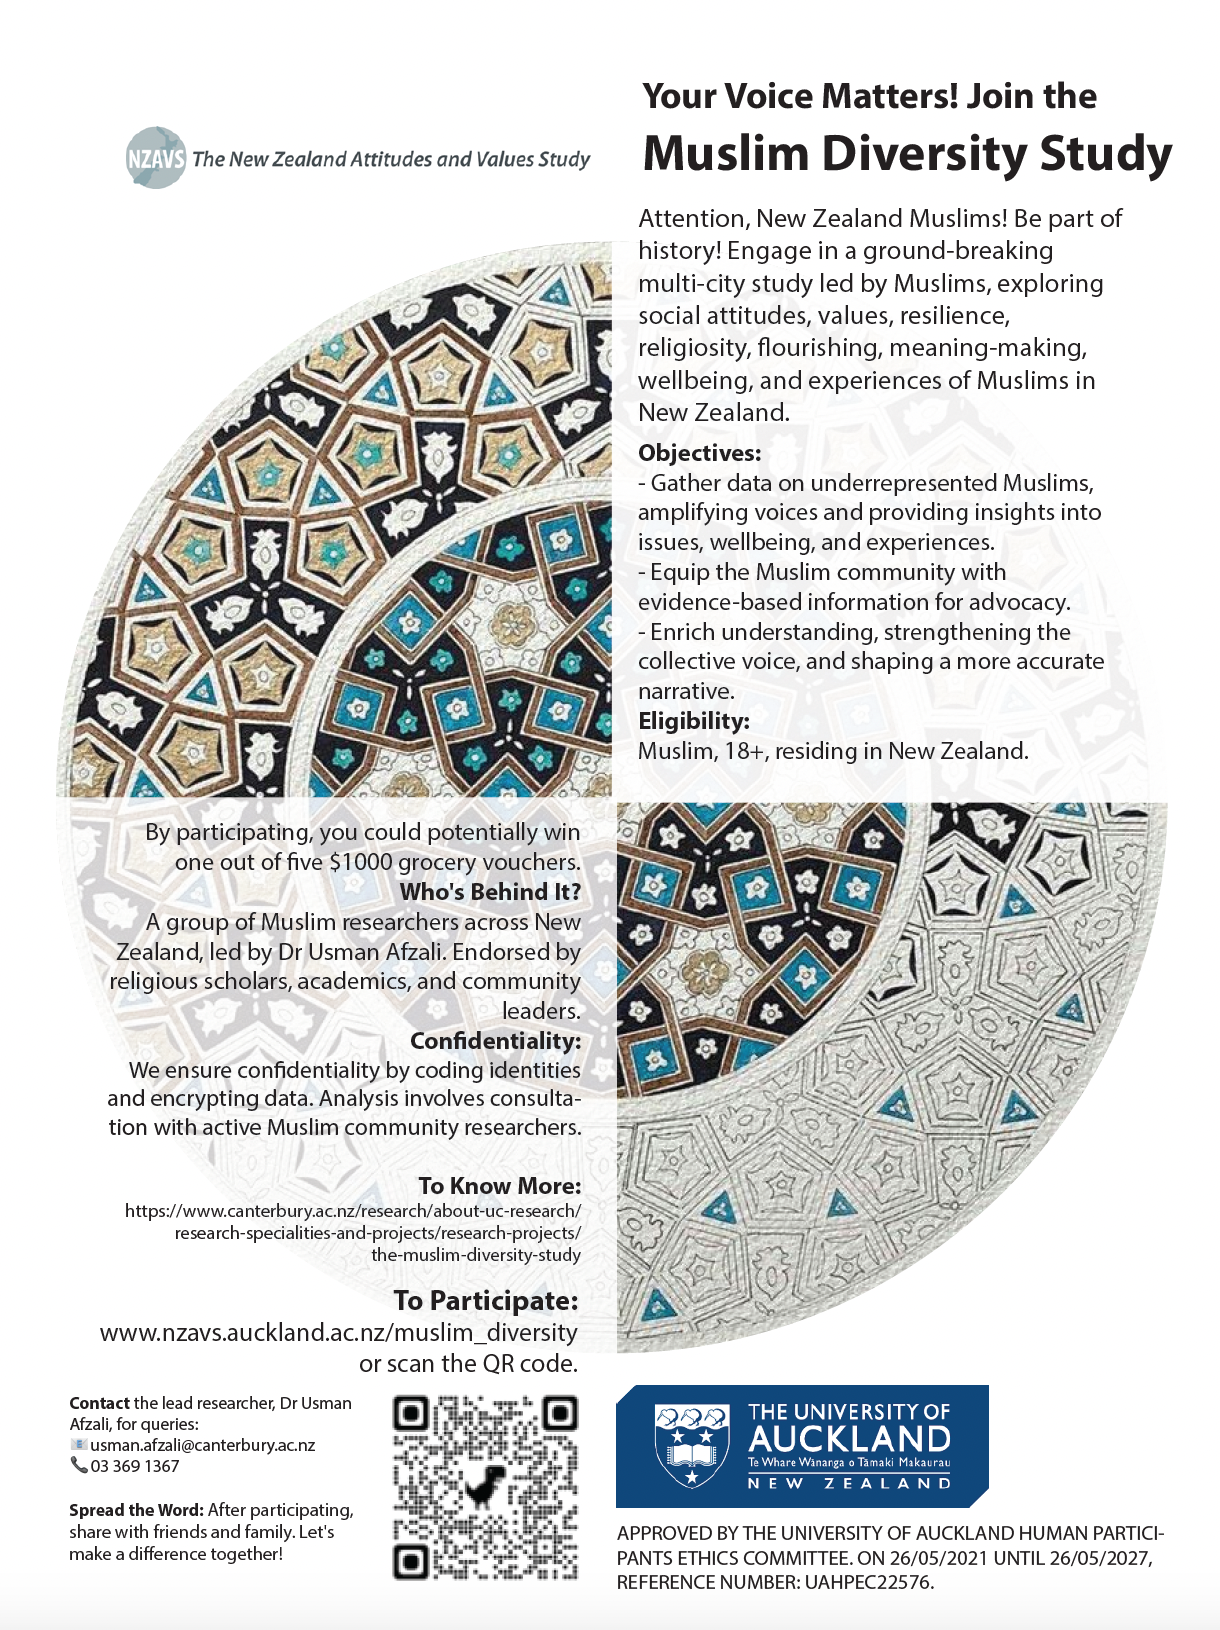
\includegraphics[width=0.8\textwidth,height=\textheight]{figs/flyer-v1.png}

}

\caption{\label{fig-appendfig}MDS Flyer}

\end{figure}%

\newpage{}

\section{Appendix E}\label{appendix-e}

\begin{figure}

\centering{

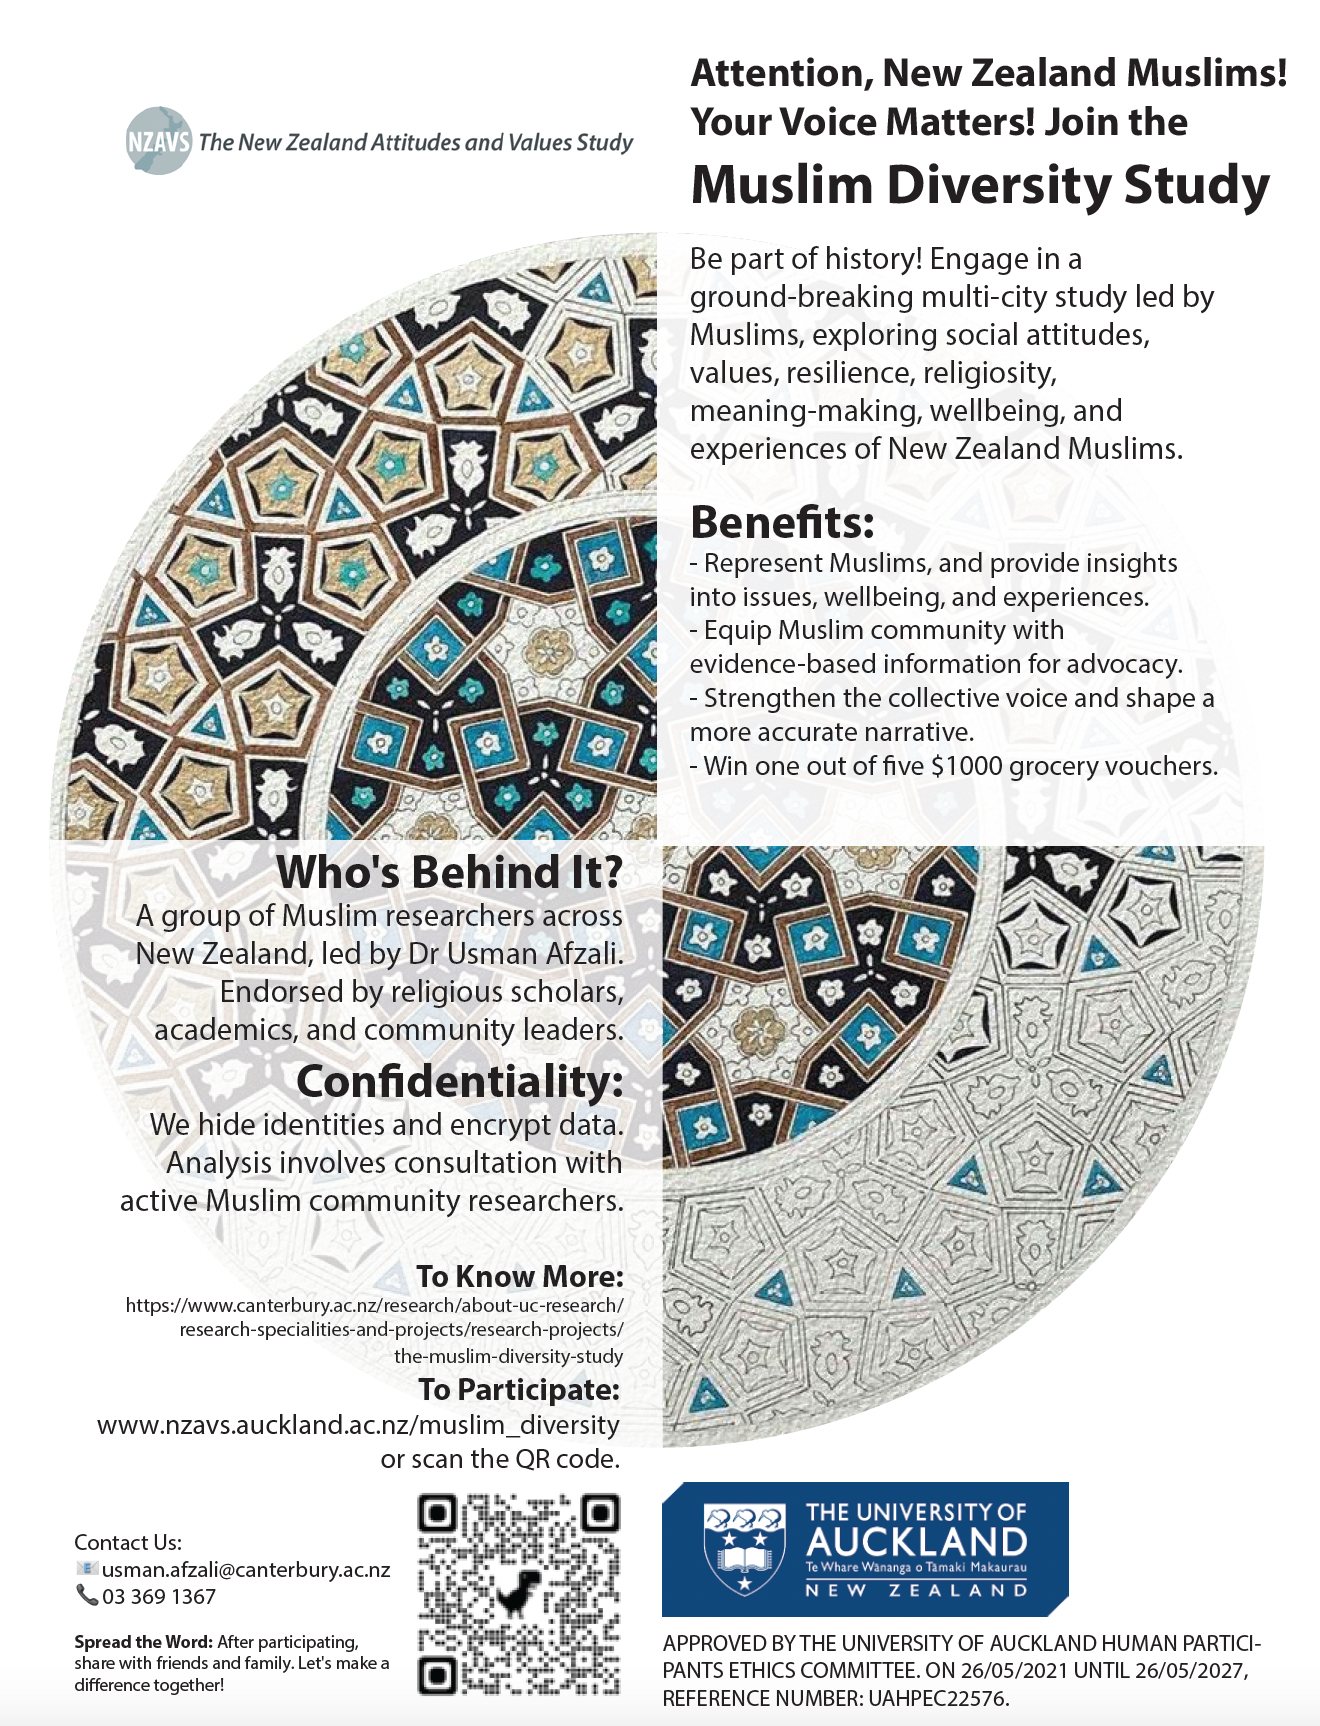
\includegraphics[width=0.8\textwidth,height=\textheight]{figs/poster-v1.png}

}

\caption{\label{fig-appendfig1}MDS Poster}

\end{figure}%

\newpage{}

\section{Appendix F}\label{appendix-f}

\subsection{MDS Vision}\label{mds-vision}

The NZAVS is committed to the following three principles for the Muslim
Diversity Study.

\noindent Protection: The NZAVS is strongly committed to respecting and
protecting data gathered from all participants and takes confidentiality
seriously. Our commitment to participant privacy and safety is central
to the NZAVS.

\noindent Participation: The NZAVS is committed to enhancing the
research capacity of our communities in Aotearoa New Zealand. Any NZAVS
research focusing specifically on the Muslim community will be reviewed
by our Muslim academic advisor Dr Usman Afzali, and/or appropriate
nominated reviewers from the Muslim community in New Zealand. We are
committed to Muslim community-led research for Muslim-focussed studies
to ensure respectful reporting that considers the social, religious, and
cultural settings of New Zealand's Muslims.

\noindent Partnership: The NZAVS actively fosters opportunities for
collaborative research with emerging Muslim researchers in New Zealand.
We seek to mentor Muslim graduate students interested in accessing NZAVS
data for research in their own postgraduate theses or dissertations. We
invite students from the Muslim community in New Zealand to contact our
Muslim academic advisor, or any member of the NZAVS board or leadership
team for guidance in developing a project.

\newpage{}

\section{Appendix G}\label{appendix-g}

\subsection{Participant
confidentiality}\label{participant-confidentiality}

\noindent Here at the NZAVS we take our participants' confidentiality
very seriously. All personal details are encrypted and stored separately
from questionnaire data. Only Professor Chris Sibley and trusted
research assistants working on the NZAVS in secure conditions have
access to participants' contact details. Participants' contact details
are used solely for the purposes of contacting them to continue their
participation in the NZAVS each year and to provide them with
information and feedback about research findings from the NZAVS.

\noindent Reference: \url{https://osf.io/75snb/wiki/home/}

\subsection{Ethics approval}\label{ethics-approval}

\noindent The Muslim Diversity Study is regulated by the University of
Auckland Human Participants Ethics Committee.

\noindent The current ethics approval statement for the 2021-2027 period
is as follows: The New Zealand Attitudes and Values Study was approved
by the University of Auckland Human Participants Ethics Committee on
26/05/2021 until 26/05/2024, and renewed on 02/05/2023 until 26/05/2027.
Reference Number: UAHPEC22576.

\noindent For any queries regarding ethical concerns, you may contact
the Chair, University of Auckland Human Participants Ethics Committee,
Ethics and Integrity Team, University of Auckland, Private Bag 92019,
Auckland 1142. Telephone 09 373-7599 ext. 83711. Email:
\href{mailto:humanethics@auckland.ac.nz}{\nolinkurl{humanethics@auckland.ac.nz}}.

\subsection{Why we need ethics
approval?}\label{why-we-need-ethics-approval}

\noindent Ethical approval for research is essential to ensure that
studies involving human participants are conducted in a morally
responsible and respectful manner. It serves to protect the rights,
wellbeing, dignity, and confidentiality of those involved in the
research, as well as the broader community affected by the study.
Ethical approval ensures that potential risks are minimized, benefits
are maximized, informed consent is obtained, and any potential conflicts
of interest or biases are addressed. This oversight helps maintain
public trust in the scientific community and upholds the fundamental
principles of fairness, respect, and accountability in research
endeavours.

\newpage{}

\section{Appendix H}\label{appendix-h}

\section{MDS Cover Letter}\label{mds-cover-letter}

\noindent Salaam alaikum, kia ora, and greetings!

\noindent My name is Dr Usman Afzali, and I am the lead researcher of
the Muslim Diversity Study. The Muslim Diversity Study is conducted as
part of the New Zealand Attitudes and Values Study. This is a broad
longitudinal study aiming to survey people from all across New Zealand
(see the information sheet on the next page for more details).

\noindent As a researcher and committed member of the New Zealand Muslim
community, I recognise the importance of including our voices in
discussions about New Zealand. This inspired me to develop a booster
study to enhance Muslim representation in the New Zealand Attitudes and
Values Study, since we are underrepresented at present. I would be
deeply grateful if you would consider participating in this survey. By
sharing your perspectives, you will enrich our understanding of the
attitudes, values, and wellbeing of the Muslim community in New Zealand.
This will strengthen the voice of our community within New Zealand. We
will publish the findings of our work in scientific journals, create
brief reports and infographics, and present our findings to Muslim
communities across New Zealand over the coming years.

\noindent My research team includes Muslim researchers from across New
Zealand. By completing this survey, you are contributing to a research
project led by people from the Muslim community for the Muslim community
in New Zealand. Furthermore, analysis of the collected data, with a
specific focus on the Muslim community, will not proceed without seeking
consultation with researchers who are themselves part of the Muslim
community.

\noindent As the survey is designed for the general New Zealand
population, there may be questions that do not necessarily apply to you.
Please feel free to skip any questions that you do not wish to answer.
This study is funded by a research grant from a not-for-profit
organisation, the Templeton Religion Trust, to help increase the
participation of Muslims in the New Zealand Attitudes and Values Study.

\begin{tcolorbox}[enhanced jigsaw, left=2mm, opacityback=0, toprule=.15mm, leftrule=.75mm, colframe=quarto-callout-color-frame, arc=.35mm, bottomrule=.15mm, breakable, colback=white, rightrule=.15mm]

If you would like to complete this questionnaire online instead of
returning by post, please use:
\url{https://www.nzavs.auckland.ac.nz/muslim_diversity}.

\end{tcolorbox}

\noindent If you have any questions or concerns regarding the Muslim
Diversity Study, please do not hesitate to reach out to me, Dr Usman
Afzali (contact details below). For general inquiries about the New
Zealand Attitudes and Values Study, please contact Professor Chris
Sibley (contact details below).

\noindent If you need help with understanding items of this
questionnaire, feel free to reach out. Our researcher assistants are
trained and have a detailed understanding of the questionnaire. Details
are available at:
\url{https://www.canterbury.ac.nz/science/schools/psyc-speech-hear/research/muslim-diversity/}

\noindent Your participation in this survey is highly valuable, and your
input will significantly contribute to our understanding of the social
values and attitudes of the Muslim community in New Zealand.

\noindent Sincerely,

Dr Usman Afzali,

School of Psychology, Speech and Hearing,

University of Canterbury, Private Bag 4800, Christchurch 8140.

(email address and phone number)

Professor Chris Sibley,

School of Psychology,

University of Auckland,

Private Bag 92019, Auckland 1142.

(email address)

\noindent APPROVED BY THE UNIVERSITY OF AUCKLAND HUMAN PARTICIPANTS
ETHICS COMMITTEE ON 26/05/2021 UNTIL 26/05/2027, REFERENCE NUMBER:
UAHPEC22576.



\end{document}
